%yright 2007, 2008, 2009 Elsevier Ltd
%% 
%% This file is part of the 'Elsarticle Bundle'.
%% ---------------------------------------------
%% 
%% It may be distributed under the conditions of the LaTeX Project Public
%% License, either version 1.2 of this license or (at your option) any
%% later version.  The latest version of this license is in
%%    http://www.latex-project.org/lppl.txt
%% and version 1.2 or later is part of all distributions of LaTeX
%% version 1999/12/01 or later.
%% 
%% The list of all files belonging to the 'Elsarticle Bundle' is
%% given in the file `manifest.txt'.
%% 

%% Template article for Elsevier's document class `elsarticle'
%% with numbered style bibliographic references
%% SP 2008/03/01

% \documentclass[preprint,11pt]{elsarticle}
\documentclass[final,1p,11pt]{elsarticle}

%\documentclass[final,1p,times]{elsarticle}


%% Use the option review to obtain double line spacing
%%\documentclass[authoryear,preprint,review,12pt]{elsarticle}

%% Use the options 1p,twocolumn; 3p; 3p,twocolumn; 5p; or 5p,twocolumn
%% for a journal layout:
%% \documentclass[final,1p,times]{elsarticle}
%% \documentclass[final,1p,times,twocolumn]{elsarticle}
%% \documentclass[final,3p,times]{elsarticle}
%% \documentclass[final,3p,times,twocolumn]{elsarticle}
%% \documentclass[final,5p,times]{elsarticle}
%% \documentclass[final,5p,times,twocolumn]{elsarticle}

%%% For including figures, graphicx.sty has been loaded in
%% elsarticle.cls. If you prefer to use the old commands
%% please give \usepackage{epsfig}


\usepackage{epsfig}
%\usepackage{cite}
%\usepackage{mcite}
\usepackage{array,tabularx,epsfig,mathrsfs,graphicx,rotating}
\usepackage{ifthen}
\usepackage{amsfonts}
\usepackage{ragged2e}
\PassOptionsToPackage{hyphens}{url}
\usepackage[hyphens]{url}
\usepackage{hyperref}
\usepackage{listings}
\usepackage{subfigure}
\usepackage{epstopdf}
% Custom colors
\usepackage{color}
\usepackage{float}

% to cross text
\usepackage[normalem]{ulem} % either use this (simple) or
\usepackage{soul} % use this (many fancier options)


\hypersetup{
  colorlinks=true,
  linkcolor=blue,
  citecolor=blue,
  urlcolor=blue
}




\graphicspath{{figs/}}


\pdfinfo{
   /Author (Chekanov/Demarteau)
   /Title  (Conceptual Design Studies for a CEPC Detector)
   /CreationDate (D:20160102195600)
   /Subject (PDFLaTeX)
   /Keywords (PDF;LaTeX)
}


\textheight=22cm
\textwidth=14.5cm

\newcommand{\beq}{\begin{equation}}
\newcommand{\eeq}{\end{equation}}
\newcommand{\la}{\langle}
\newcommand{\promc}{{\sc ProMC}}
\newcommand{\ra}{\rangle}
\newcommand{\eps}{\epsilon}
\newcommand{\ud}{\mathrm{d}}
\newcommand{\Ec}{\mathcal{E}}
\newcommand{\Fc}{\mathcal{F}}
\newcommand{\Za}{\mathrm{Z_1}}
\newcommand{\Zb}{\mathrm{Z_2}}
\newcommand{\Zn}{\mathrm{Z_n}}
\newcommand{\F}{\mathrm{F}}

\chardef\til=126
\newcommand{\mev}{{\,\mathrm{MeV}}}
\newcommand{\gev}{{\,\mathrm{GeV}}}
\newcommand{\tev}{{\,\mathrm{TeV}}}
\newcommand{\GEANTfour} {\textsc{geant4}}
\journal{XXX-XXX}



\begin{document}

\section{Studies of signal and background separation using calorimeter clusters}
%%In the future detector, when the energy is increased, the boost jet is bigger, and it will be more difficult to distinguish the signal and the background. In this section, we want to study different variables and see their ability to separate the signal and the background in different detector sizes in the clustering of detector-level.\\
In this section, we study different jet substructure variables and compare their ability to separate the signal and the background for different detector sizes using calorimeter clusters.\\
%%Figure 3 to 5 show the ROC curves of three variables, $c2b1$ , $\tau_{21}$, and $\tau_{32}$. For each variable, there are three different sizes of the sub-detector HCAL compared at four special collision energies. For different sizes, the one with the highest background rejection rate, which is 1-background efficiency, at the same signal efficiency has the best separate ability.

Figures \textcolor{blue}{1}--\textcolor{blue}{3} show the ROC curves of three variables, $c_2^{(1)}$~\cite{Larkoski:2013eya} , $\tau_{21}$~\cite{Thaler:2010tr}, and $\tau_{32}$~\cite{Thaler:2010tr}, respectively. Three different cell sizes of the HCAL are compared for four collision energies. For different cell sizes with the same signal efficiency, the one with the highest background rejection rate, namely (1-background efficiency), has the highest separate power.\\

In Figure \textcolor{blue}{1} for the variable $c_2^{(1)}$ , the ROC curves of the three detector cell sizes are close to each other for each collision energy. Therefore, this variable is not sensitive to the detector cell size.\\

For the $\tau_{21}$ variable in Figure \textcolor{blue}{2}, at 5 TeV, the smallest detector size (1$\times$1 cm) can separate the background from the signal well. However, this is not the usual case as the ROC curves nearly merge together at higher collision energy. In addition, the detector with the bigger size tends to have higher separation power than the smaller detector size in 20 and 40 TeV collision energy.\\

Figure \textcolor{blue}{3} shows the variable $\tau_{32}$, where the smallest detector size has the best separation power for all collision energies.\\

In conclusion, in all the cases of energy and detector size, the variable $c_2^{(1)}$ has the best separation power compared to the other two variables. In addition, the variable $\tau_{32}$ follows the expectation that smaller detector size has better separation power.\\

\label{sec:efficiency}

%25bins
\begin{figure}
\begin{center}
   \subfigure[5 TeV in cluster] {
   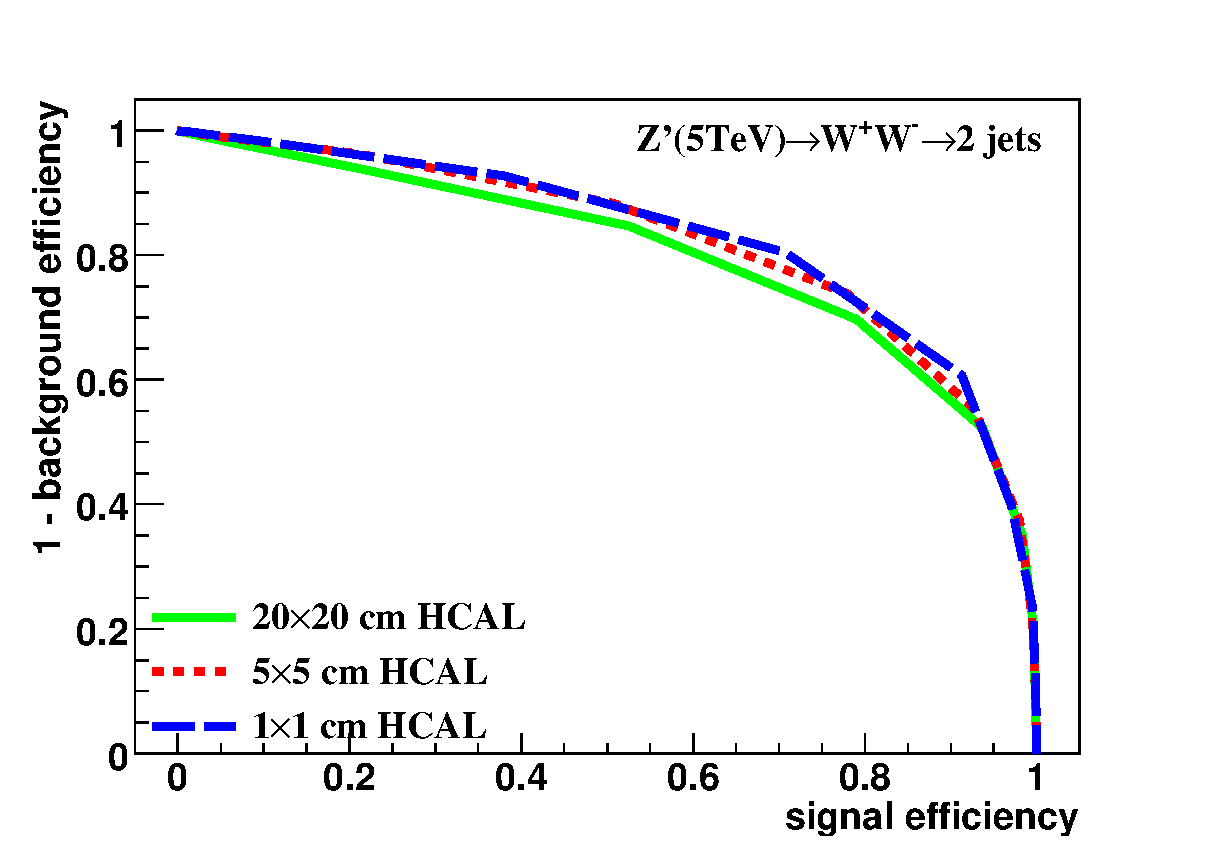
\includegraphics[width=0.43\textwidth]{figs/cluster_c2b1_5tev_04_eff.eps}\hfill
   }
   \subfigure[10 TeV in cluster] {
   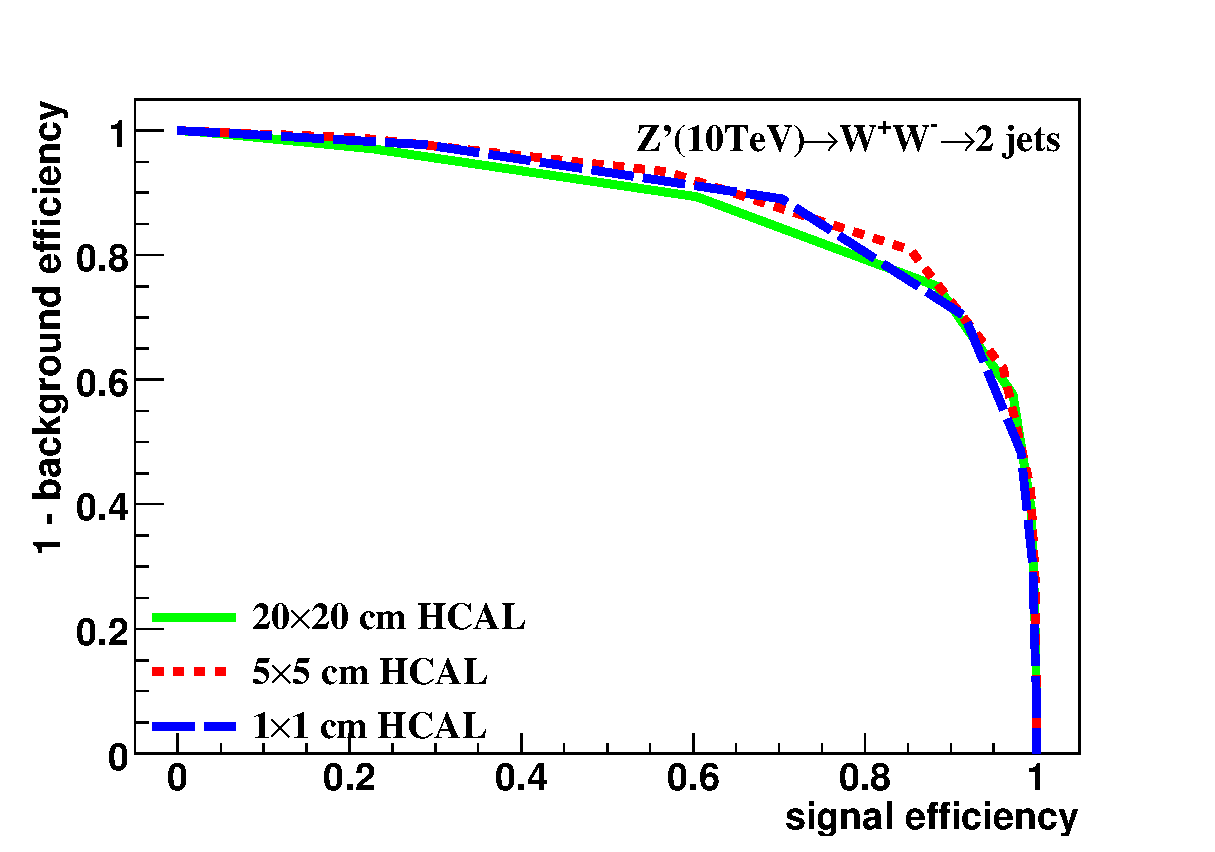
\includegraphics[width=0.43\textwidth]{figs/cluster_c2b1_10tev_04_eff.eps}
   }
   \subfigure[20 TeV in cluster] {
   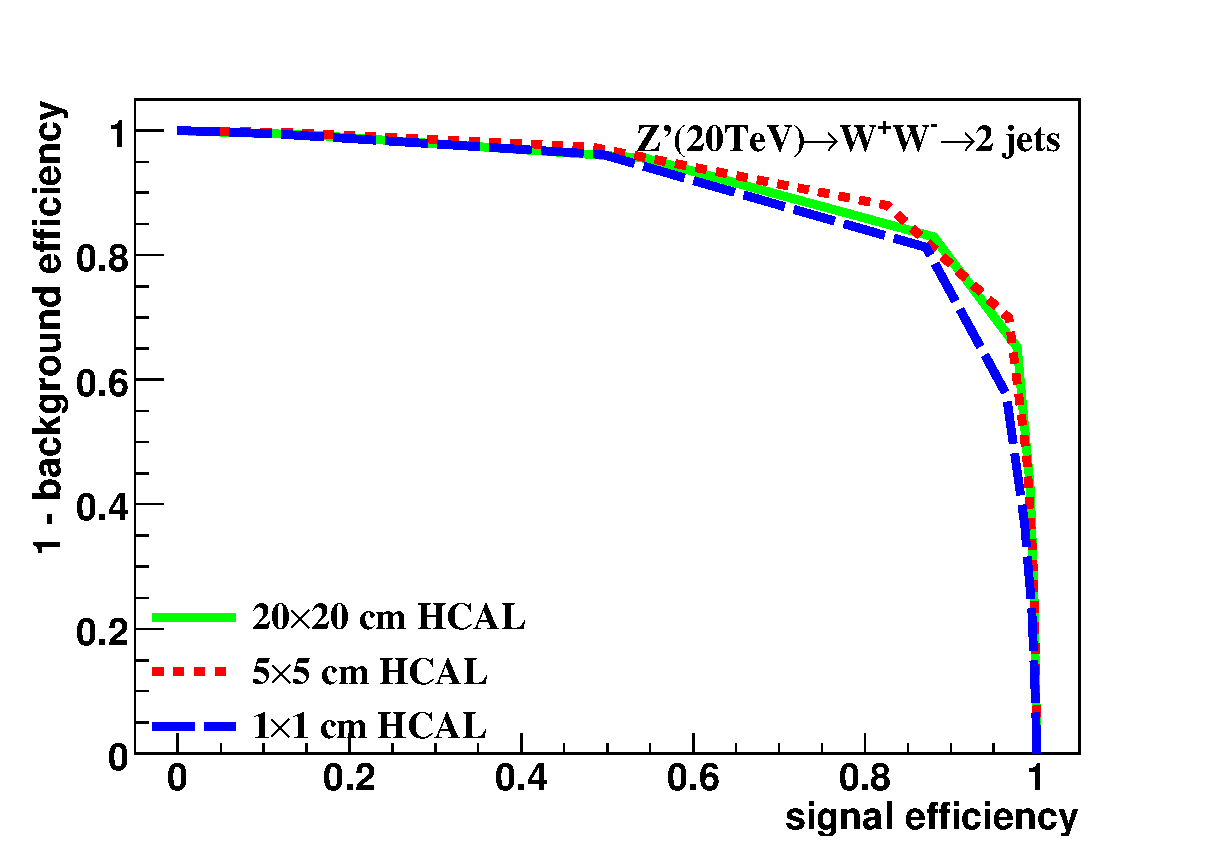
\includegraphics[width=0.43\textwidth]{figs/cluster_c2b1_20tev_04_eff.eps}
   }
   \subfigure[40 TeV in cluster] {
   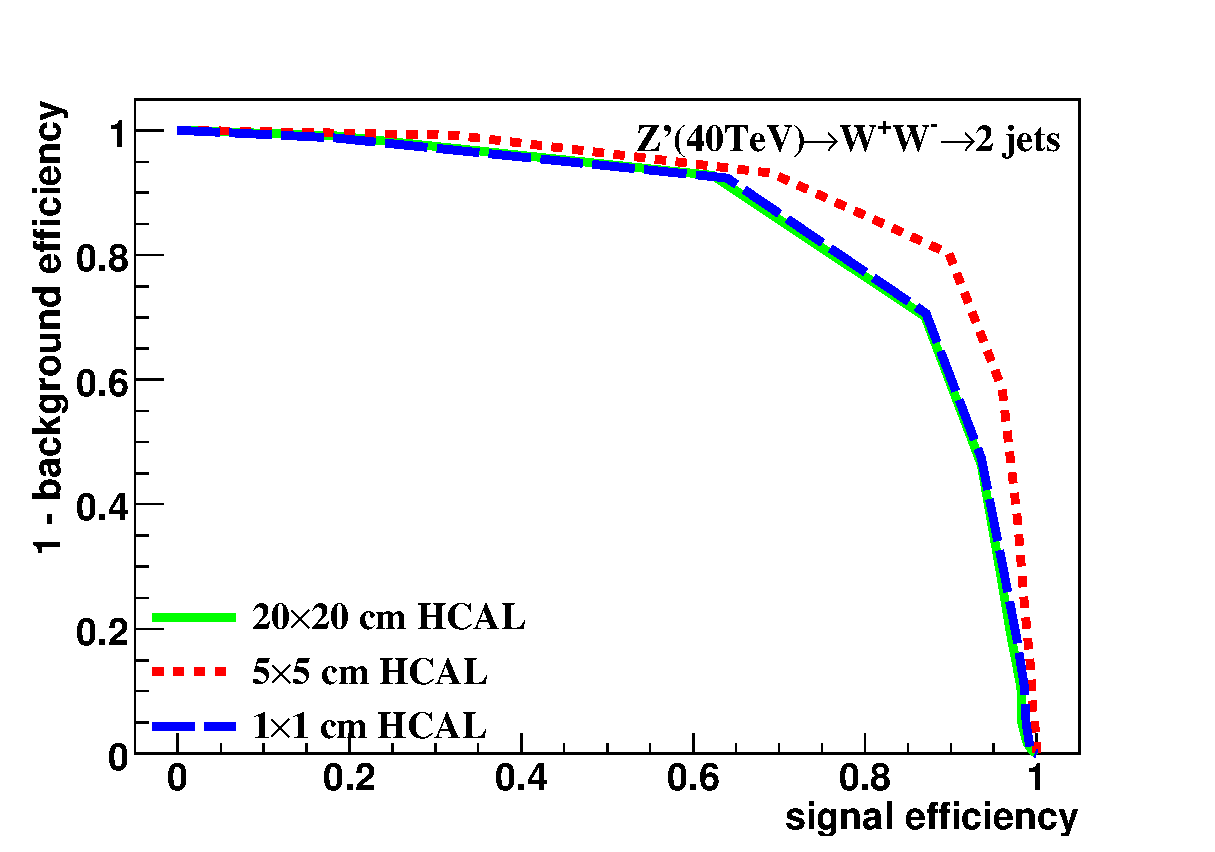
\includegraphics[width=0.43\textwidth]{figs/cluster_c2b1_40tev_04_eff.eps}
   }
\end{center}
\caption{Signal efficiency versus background rejection rate using $c_2^{(1)}$.The energies of collision at (a)5, (b)10, (c)20, (d)40TeV are shown here. In each picture, the three ROC curves correspond to different detector sizes.}
\label{fig:cluster_c2b1}
\end{figure}

%25bins
\begin{figure}
\begin{center}
   \subfigure[5 TeV in cluster] {
   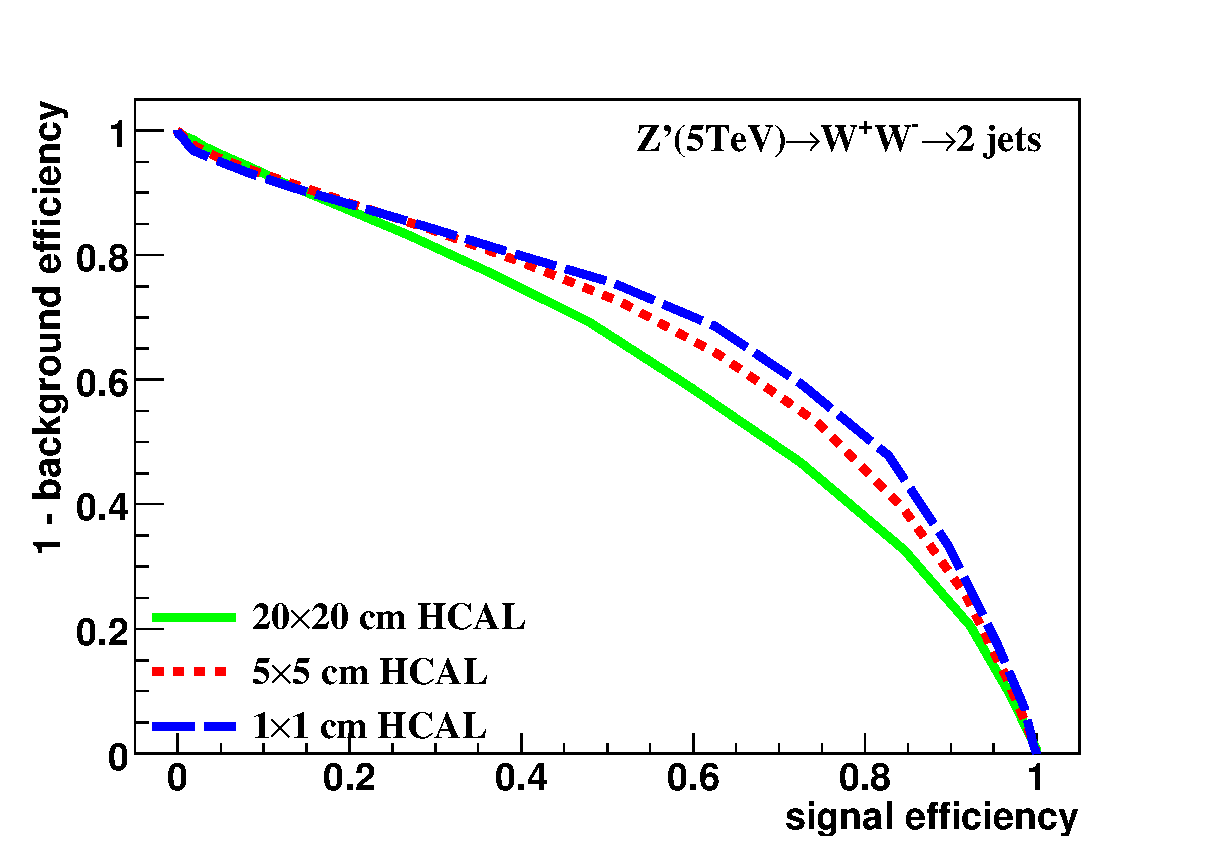
\includegraphics[width=0.43\textwidth]{figs/cluster_tau21_5tev_04_eff.eps}\hfill
   }
   \subfigure[10 TeV in cluster] {
   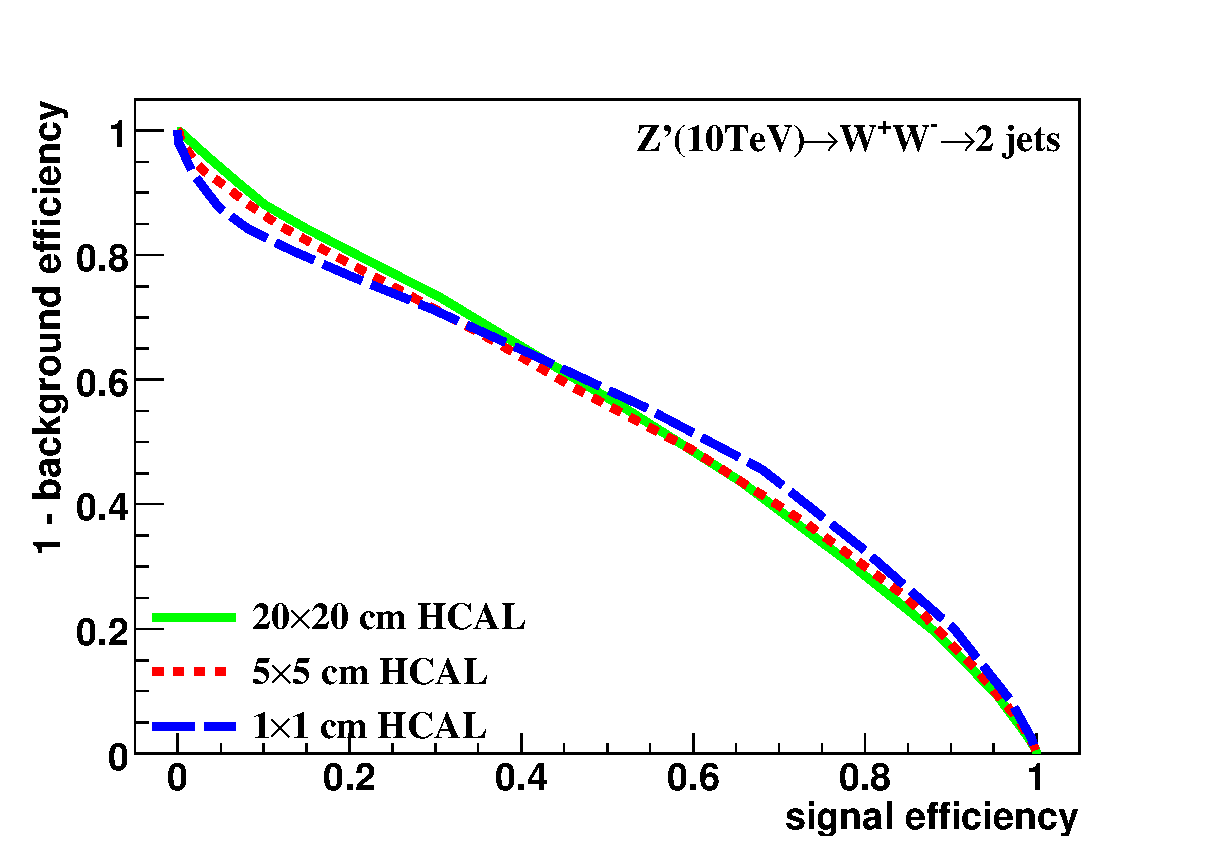
\includegraphics[width=0.43\textwidth]{figs/cluster_tau21_10tev_04_eff.eps}
   }
   \subfigure[20 TeV in cluster] {
   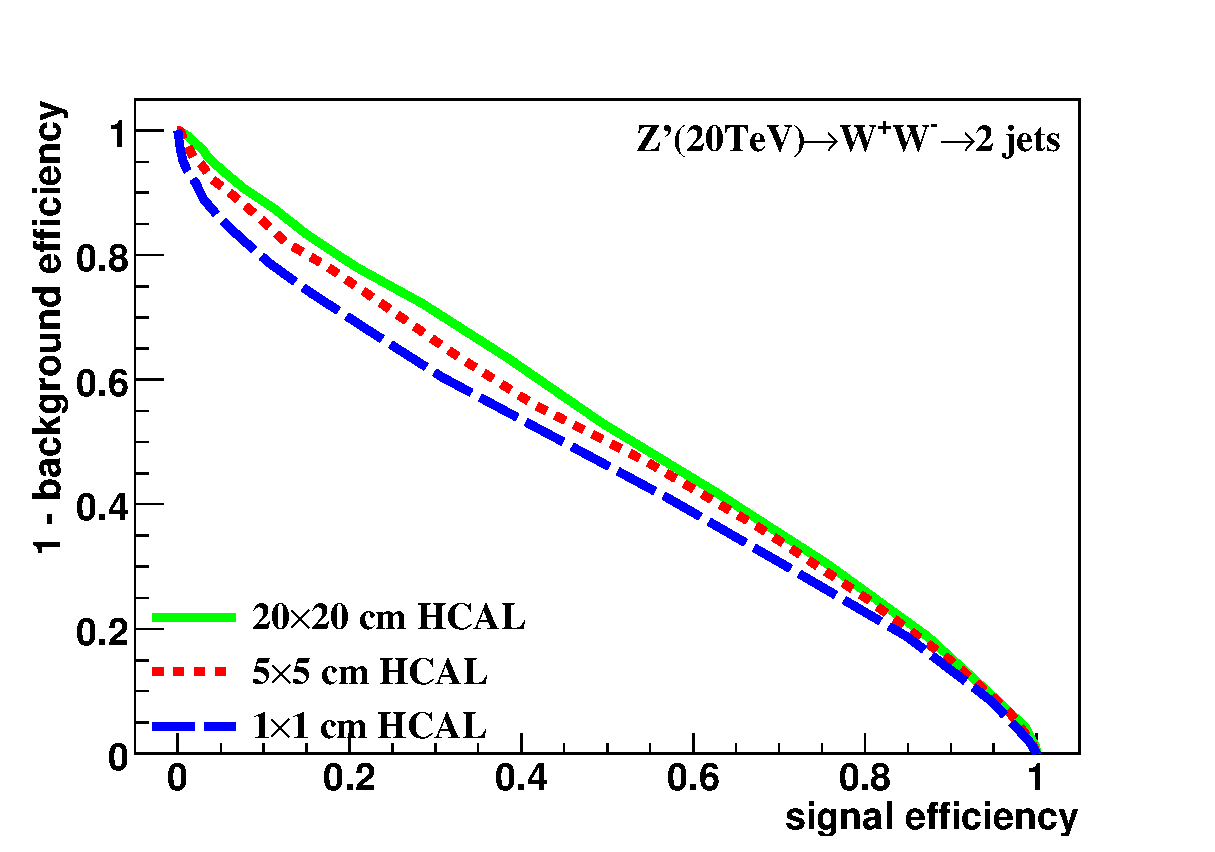
\includegraphics[width=0.43\textwidth]{figs/cluster_tau21_20tev_04_eff.eps}
   }
   \subfigure[40 TeV in cluster] {
   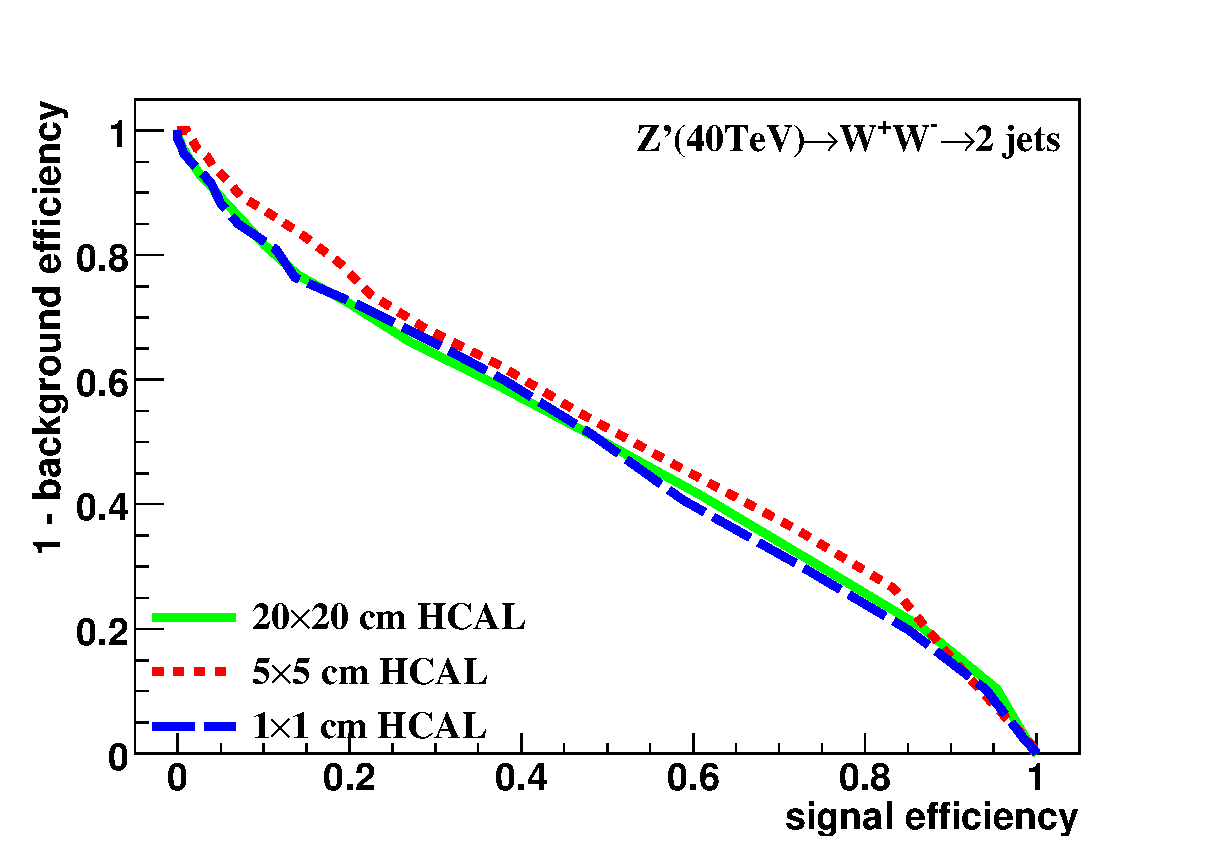
\includegraphics[width=0.43\textwidth]{figs/cluster_tau21_40tev_04_eff.eps}
   }
\end{center}
\caption{Signal efficiency versus background rejection rate using $\tau_{21}$.The energies of collision at (a)5, (b)10, (c)20, (d)40TeV are shown here. In each picture, the three ROC curves correspond to different detector sizes.}
\label{fig:cluster_tau21}
\end{figure}

%25bins
\begin{figure}
\begin{center}
   \subfigure[5 TeV in cluster] {
   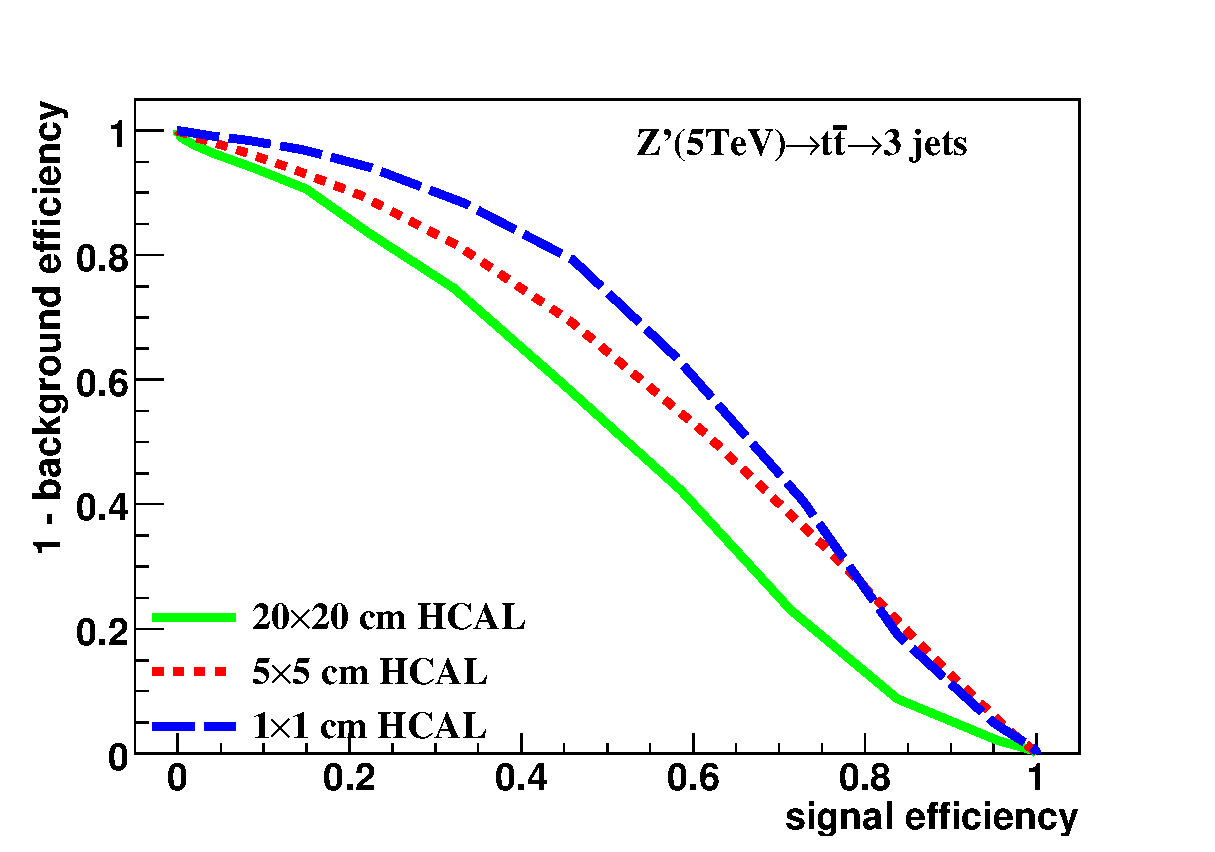
\includegraphics[width=0.43\textwidth]{figs/cluster_tau32_5tev_04_eff.eps}\hfill
   }
   \subfigure[10 TeV in cluster] {
   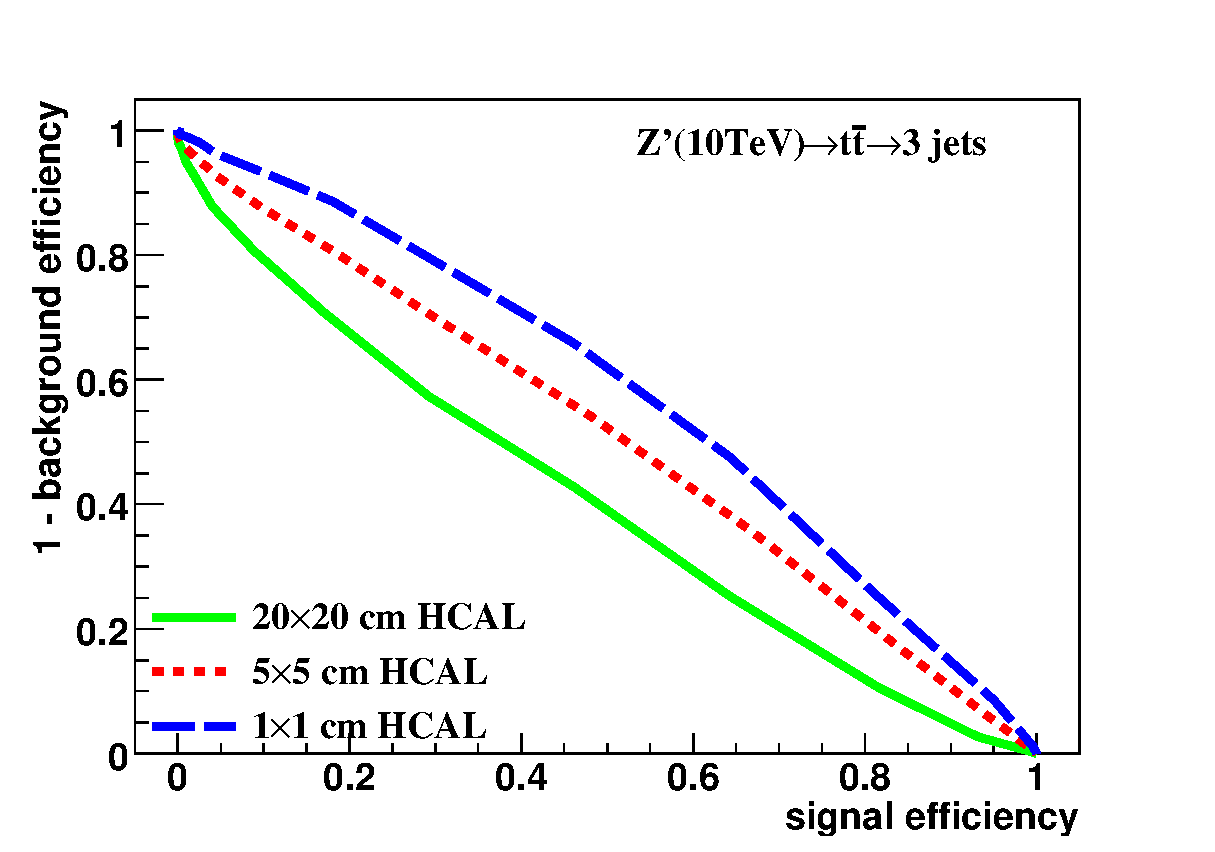
\includegraphics[width=0.43\textwidth]{figs/cluster_tau32_10tev_04_eff.eps}
   }
   \subfigure[20 TeV in cluster] {
   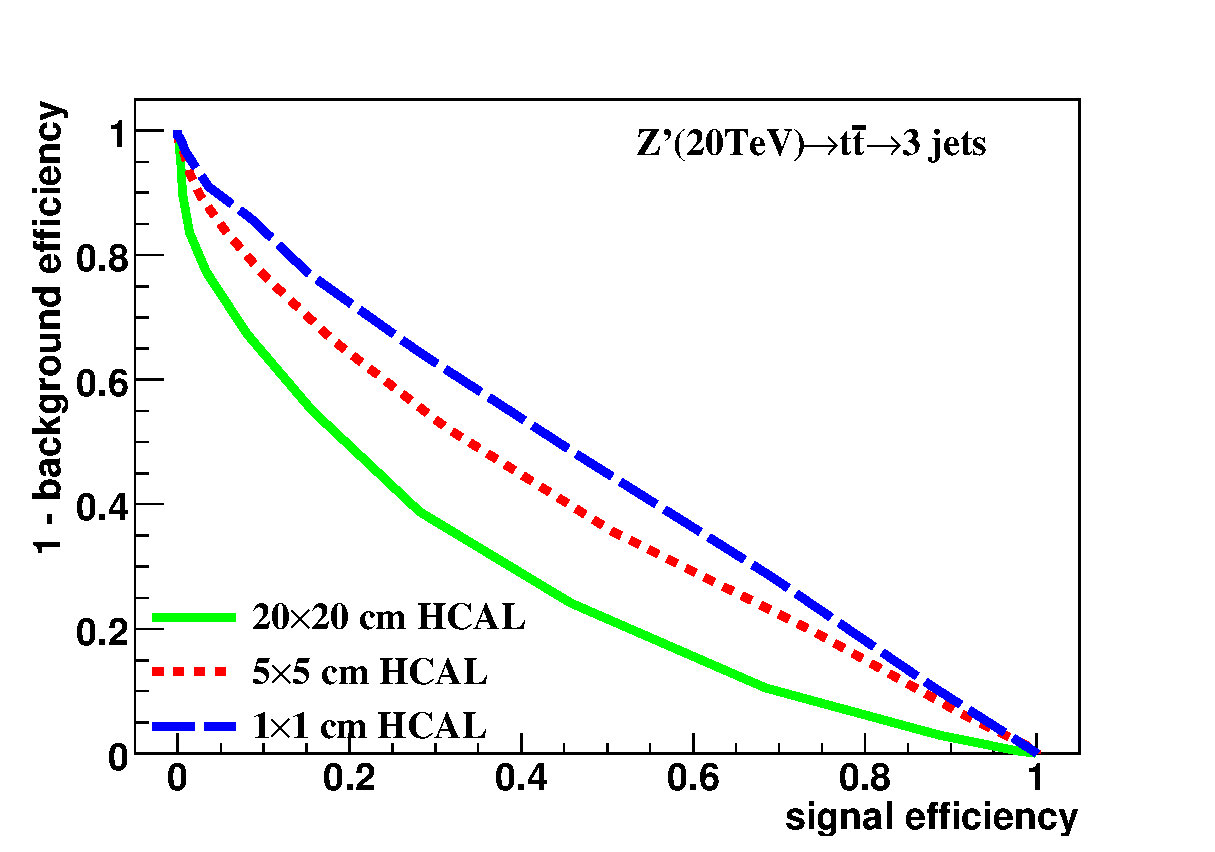
\includegraphics[width=0.43\textwidth]{figs/cluster_tau32_20tev_04_eff.eps}
   }
   \subfigure[40 TeV in cluster] {
   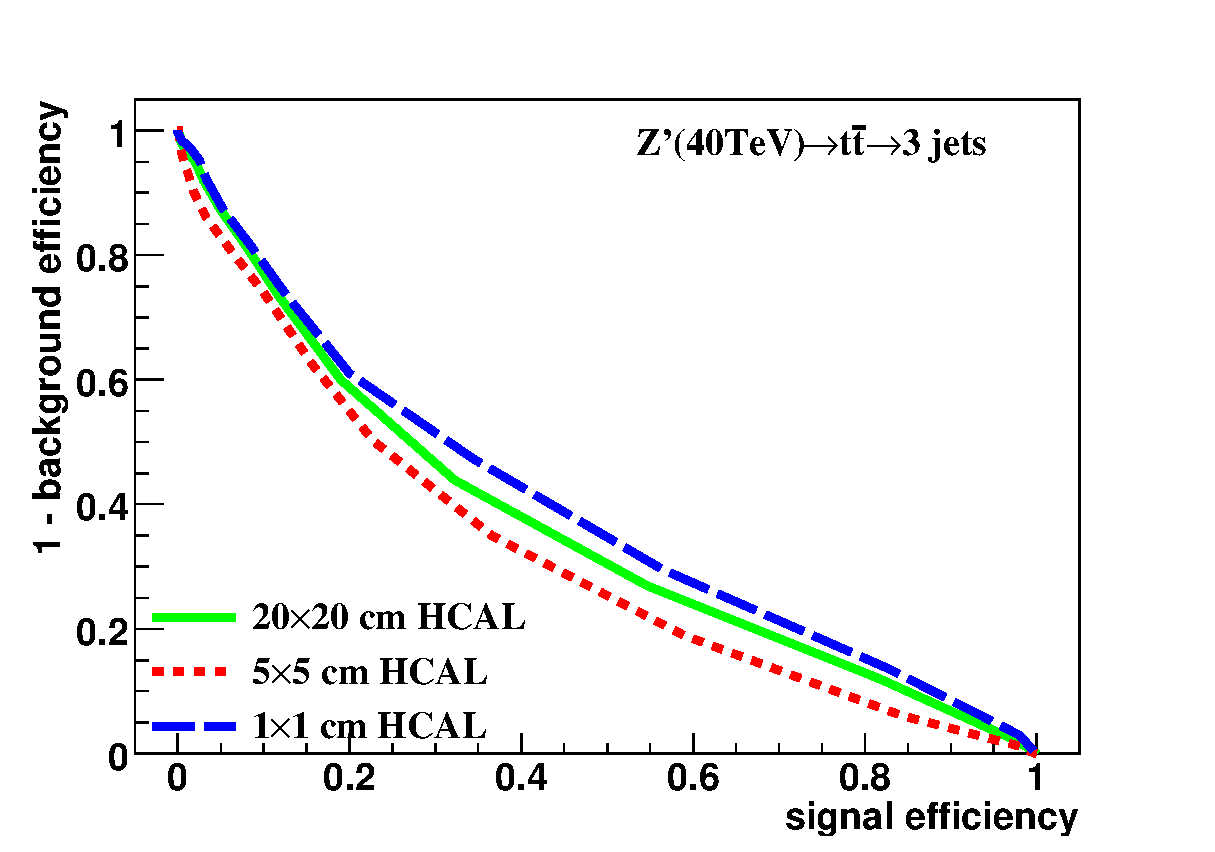
\includegraphics[width=0.43\textwidth]{figs/cluster_tau32_40tev_04_eff.eps}
   }
\end{center}
\caption{Signal efficiency versus background rejection rate using $\tau_{32}$.The energies of collision at (a)5, (b)10, (c)20, (d)40TeV are shown here. In each picture, the three ROC curves correspond to different detector sizes.}
\label{fig:cluster_tau32}
\end{figure}


\section{Studies of signal and background separation using calorimeter hit cut at 0.5GeV}

%25bins
\begin{figure}
\begin{center}
   \subfigure[5 TeV rawhit cut at 0.5GeV] {
   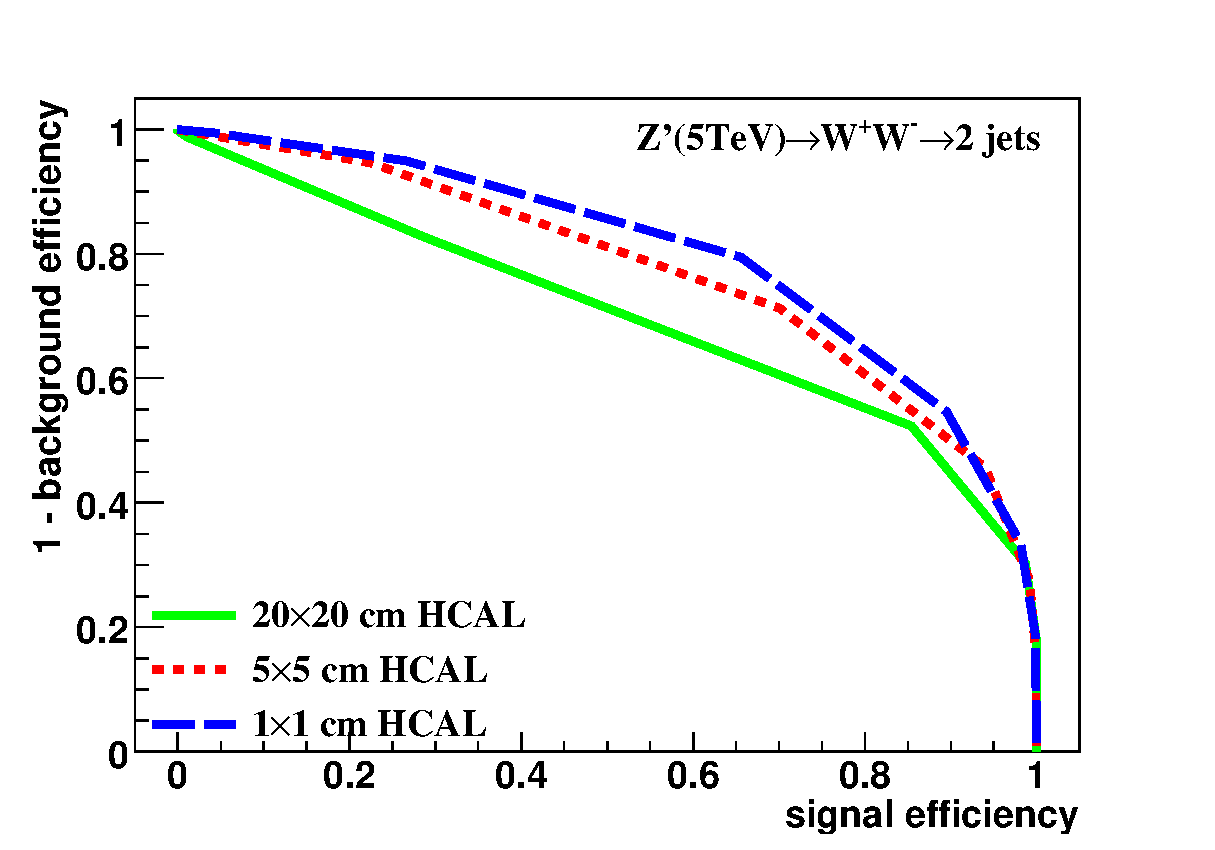
\includegraphics[width=0.43\textwidth]{figs/Rawhit_05GeV_c2b1_5tev_04_eff.eps}\hfill
   }
   \subfigure[10 TeV rawhit cut at 0.5GeV] {
   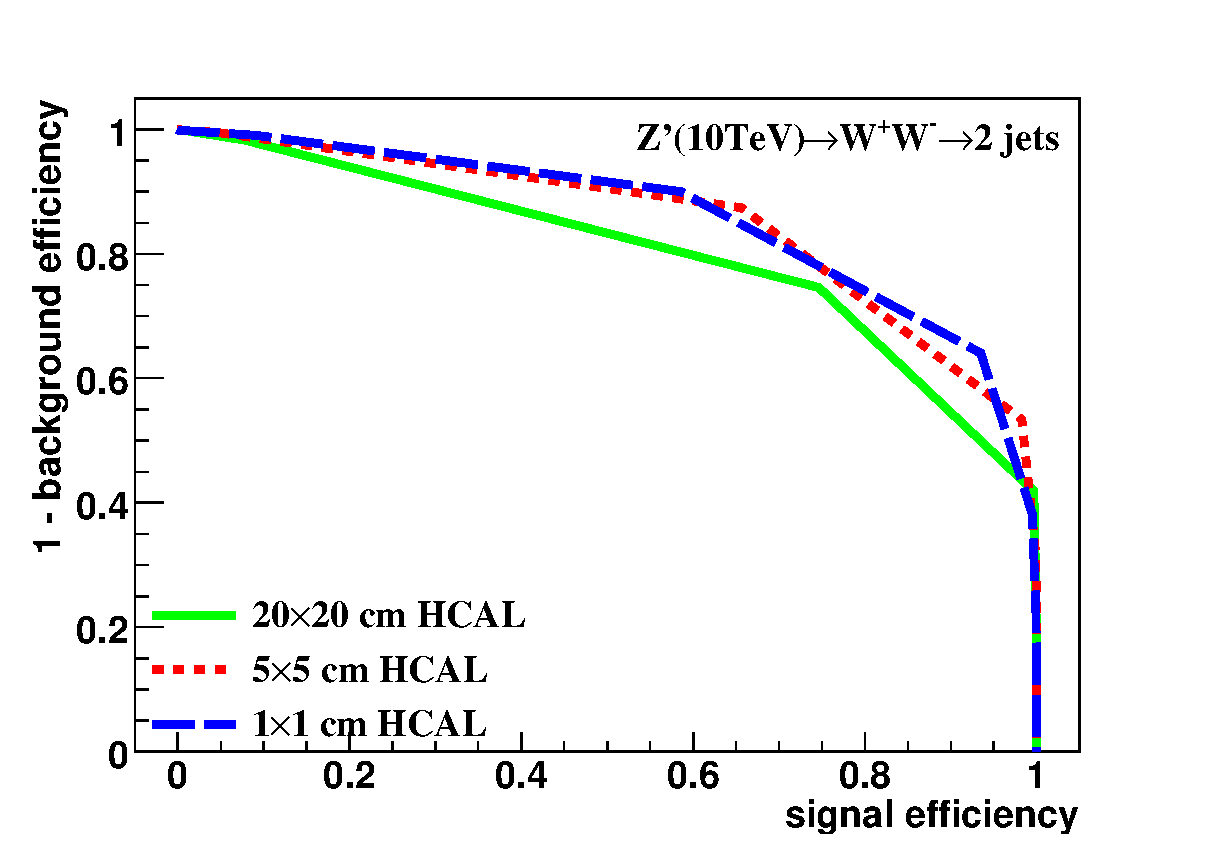
\includegraphics[width=0.43\textwidth]{figs/Rawhit_05GeV_c2b1_10tev_04_eff.eps}
   }
   \subfigure[20 TeV rawhit cut at 0.5GeV] {
   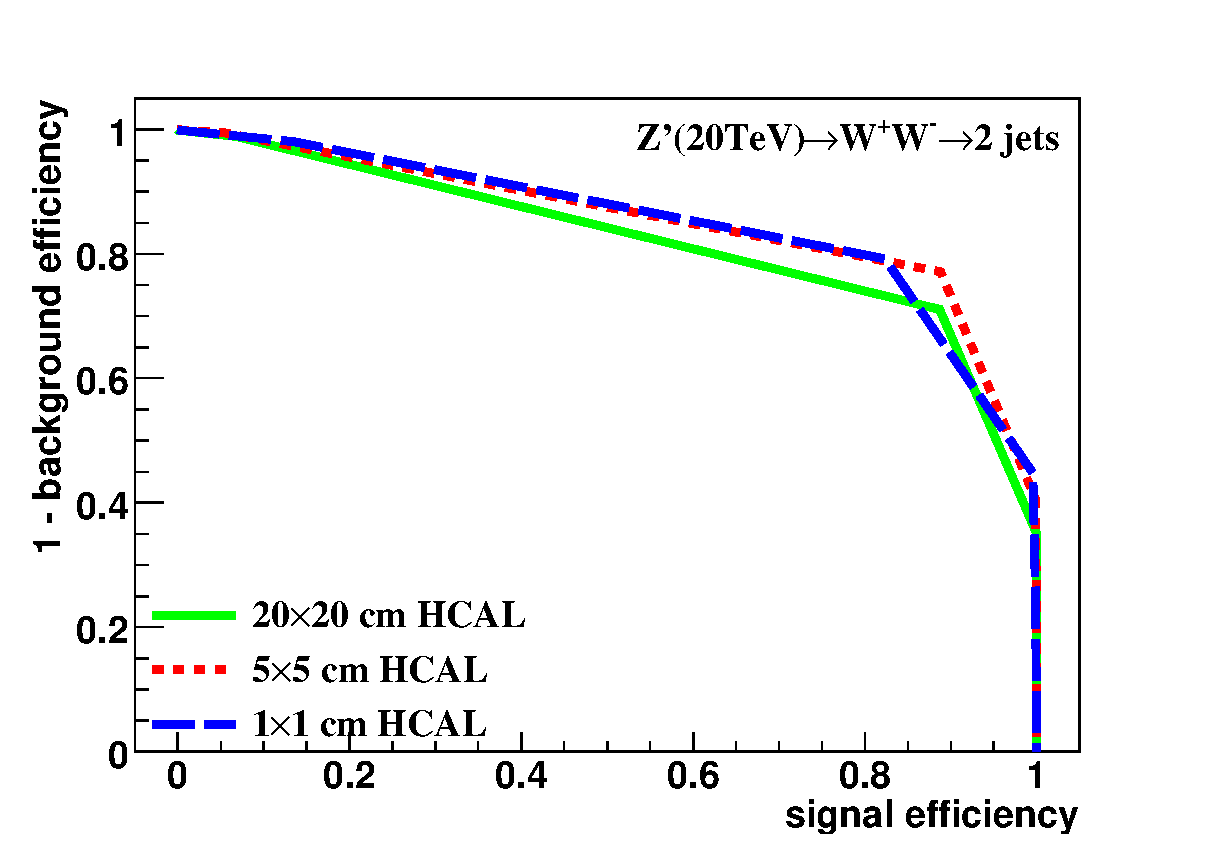
\includegraphics[width=0.43\textwidth]{figs/Rawhit_05GeV_c2b1_20tev_04_eff.eps}
   }
   \subfigure[40 TeV rawhit cut at 0.5GeV] {
   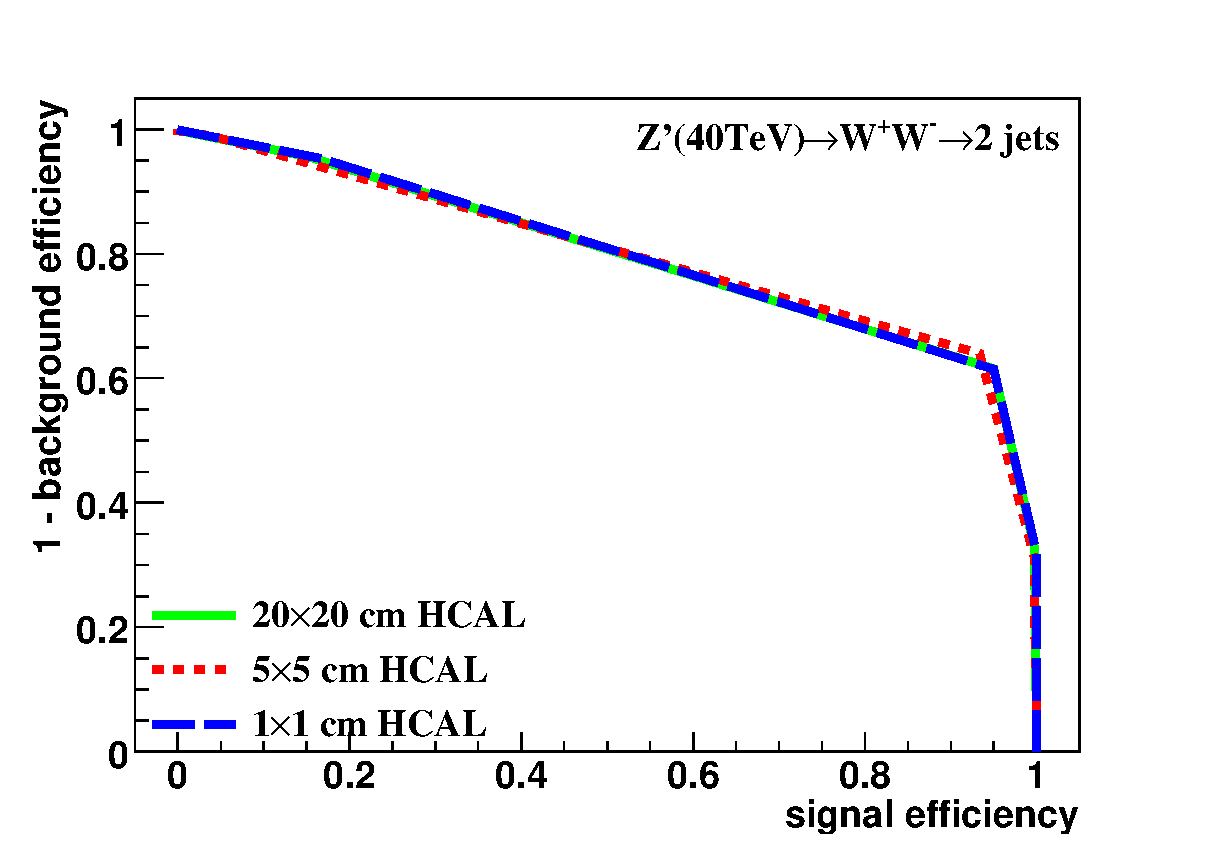
\includegraphics[width=0.43\textwidth]{figs/Rawhit_05GeV_c2b1_40tev_04_eff.eps}
   }
\end{center}
\caption{Signal efficiency versus background rejection rate using $c_2^{(1)}$.The energies of collision at (a)5, (b)10, (c)20, (d)40TeV are shown here. In each picture, the three ROC curves correspond to different detector sizes.}
\label{fig:rawhit_0.5GeV_c2b1}
\end{figure}

%25bins
\begin{figure}
\begin{center}
   \subfigure[5 TeV rawhit cut at 0.5GeV] {
   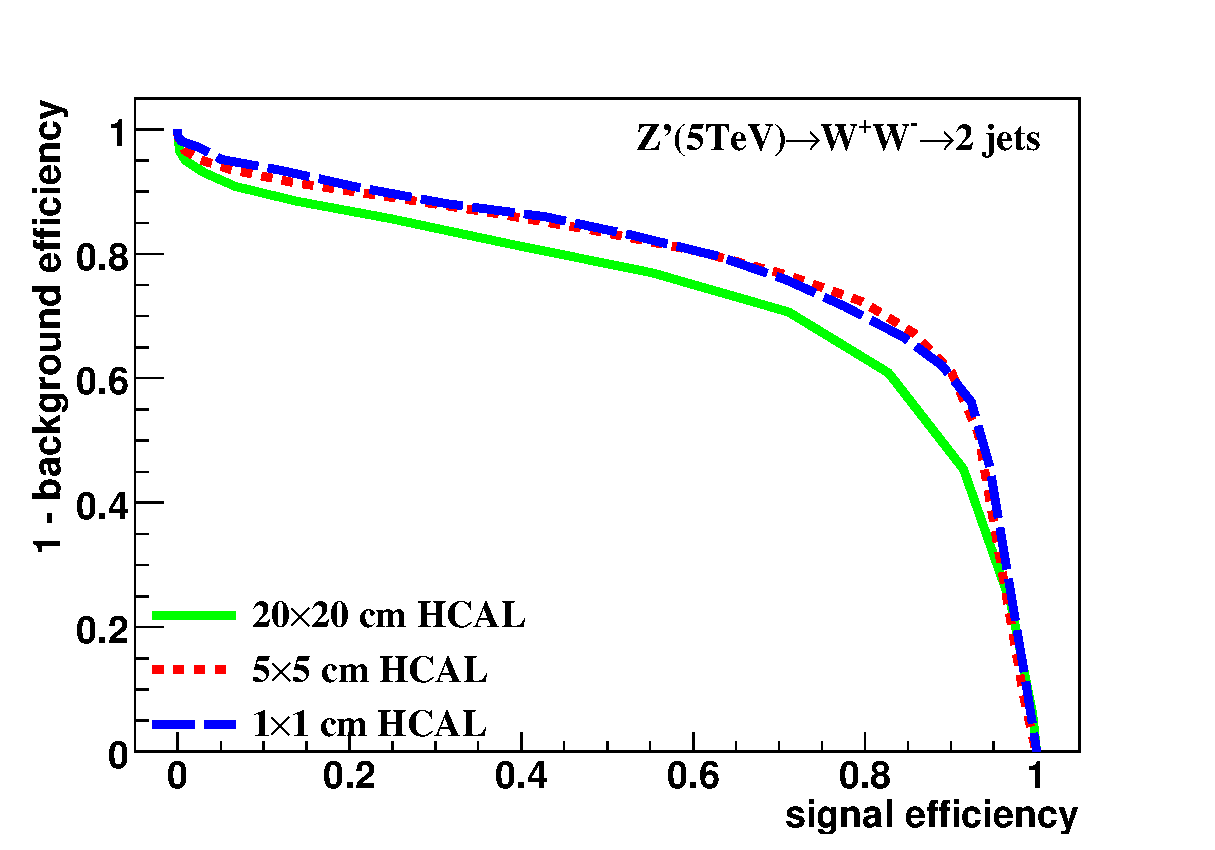
\includegraphics[width=0.43\textwidth]{figs/Rawhit_05GeV_tau21_5tev_04_eff.eps}\hfill
   }
   \subfigure[10 TeV rawhit cut at 0.5GeV] {
   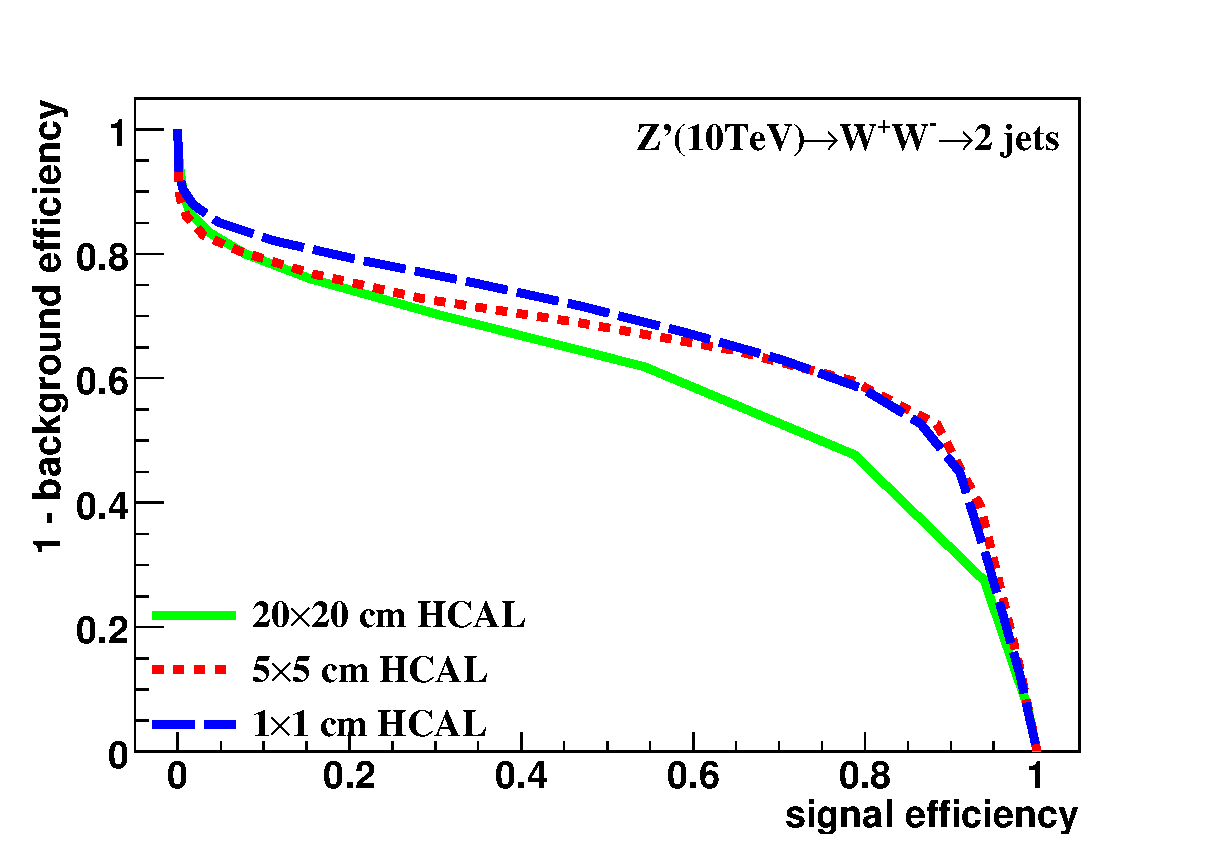
\includegraphics[width=0.43\textwidth]{figs/Rawhit_05GeV_tau21_10tev_04_eff.eps}
   }
   \subfigure[20 TeV rawhit cut at 0.5GeV] {
   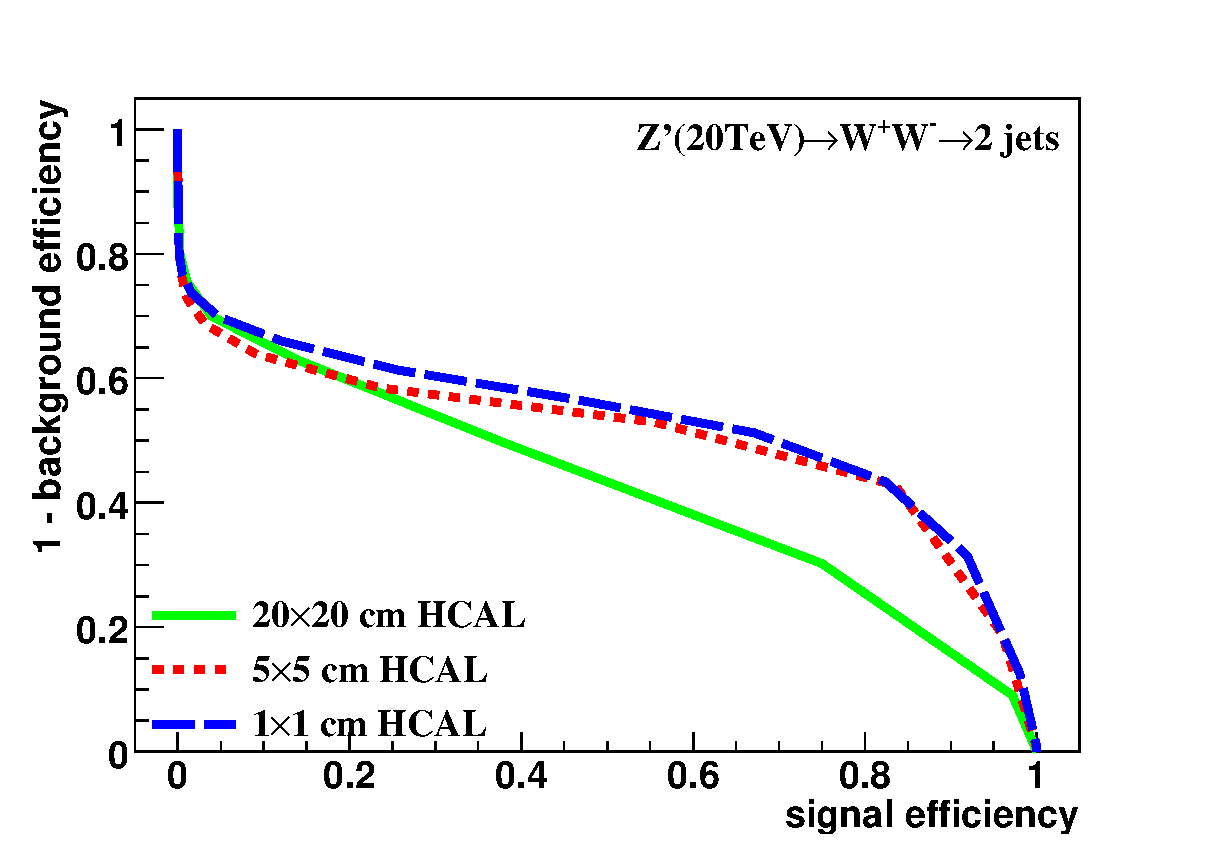
\includegraphics[width=0.43\textwidth]{figs/Rawhit_05GeV_tau21_20tev_04_eff.eps}
   }
   \subfigure[40 TeV rawhit cut at 0.5GeV] {
   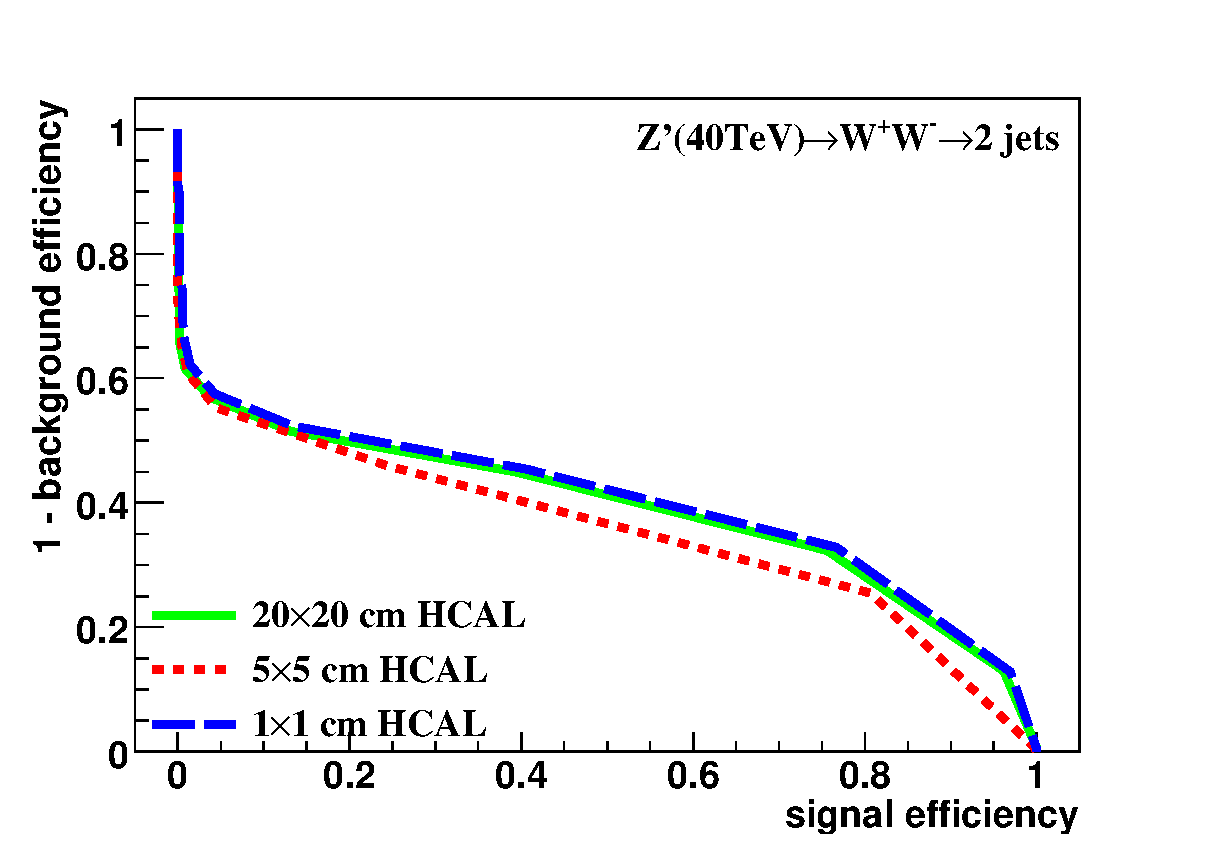
\includegraphics[width=0.43\textwidth]{figs/Rawhit_05GeV_tau21_40tev_04_eff.eps}
   }
\end{center}
\caption{Signal efficiency versus background rejection rate using $\tau_{21}$.The energies of collision at (a)5, (b)10, (c)20, (d)40TeV are shown here. In each picture, the three ROC curves correspond to different detector sizes.}
\label{fig:rawhit_0.5GeV_tau21}
\end{figure}

%25bins
\begin{figure}
\begin{center}
   \subfigure[5 TeV rawhit cut at 0.5GeV] {
   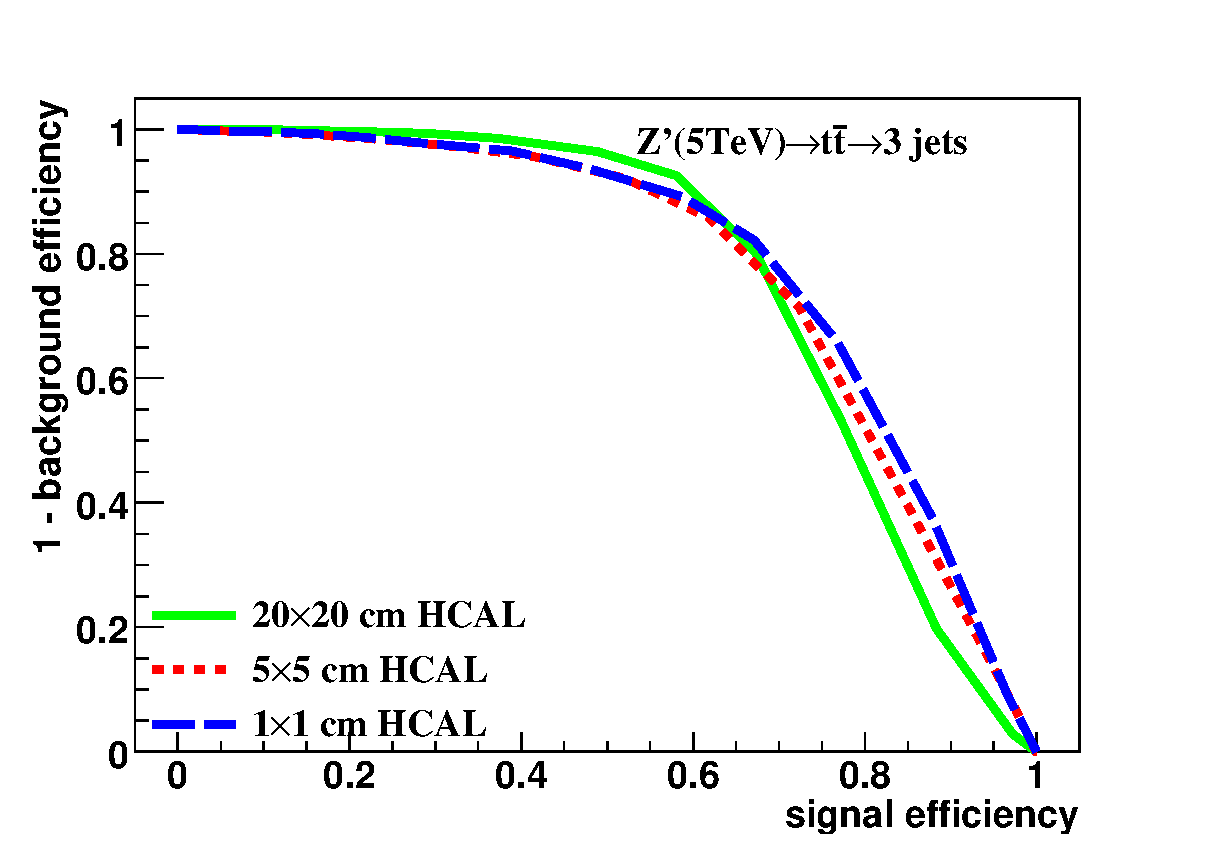
\includegraphics[width=0.43\textwidth]{figs/Rawhit_05GeV_tau32_5tev_04_eff.eps}\hfill
   }
   \subfigure[10 TeV rawhit cut at 0.5GeV] {
   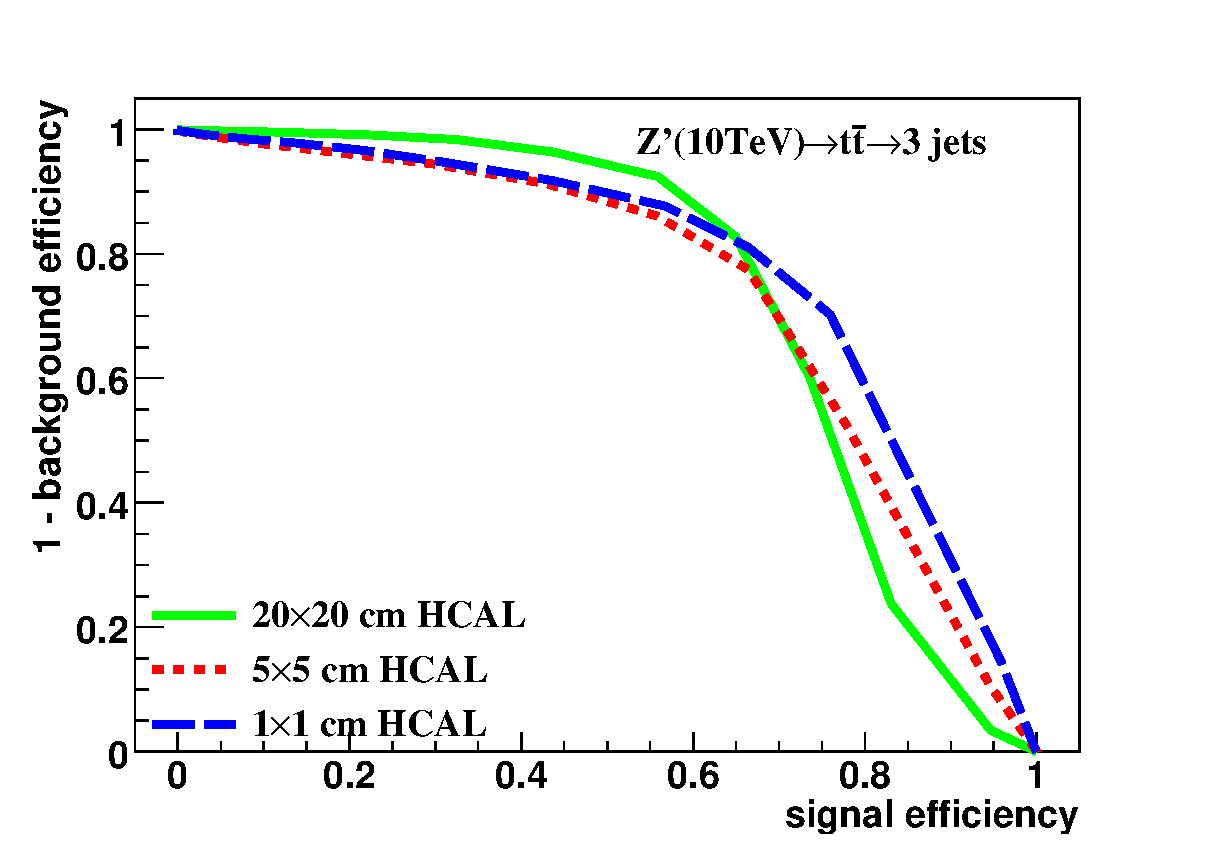
\includegraphics[width=0.43\textwidth]{figs/Rawhit_05GeV_tau32_10tev_04_eff.eps}
   }
   \subfigure[20 TeV rawhit cut at 0.5GeV] {
   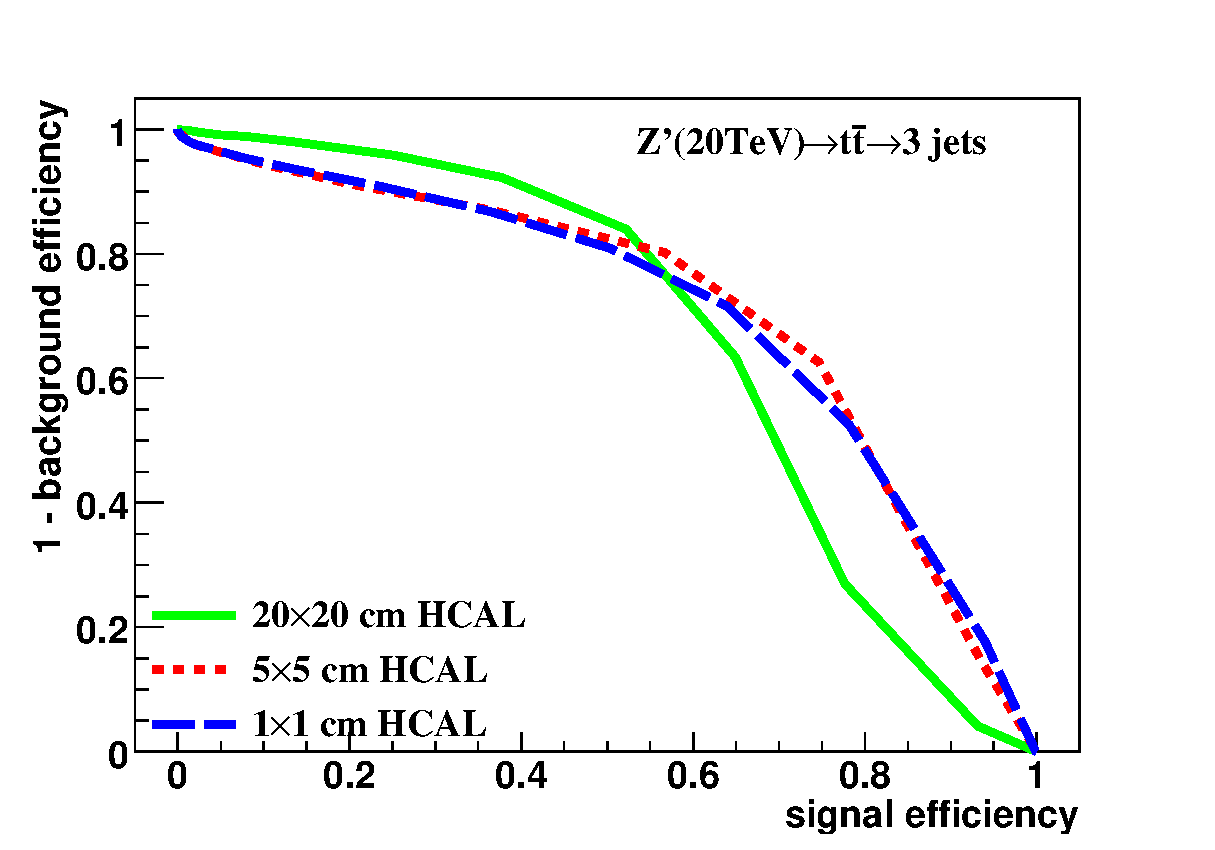
\includegraphics[width=0.43\textwidth]{figs/Rawhit_05GeV_tau32_20tev_04_eff.eps}
   }
   \subfigure[40 TeV rawhit cut at 0.5GeV] {
   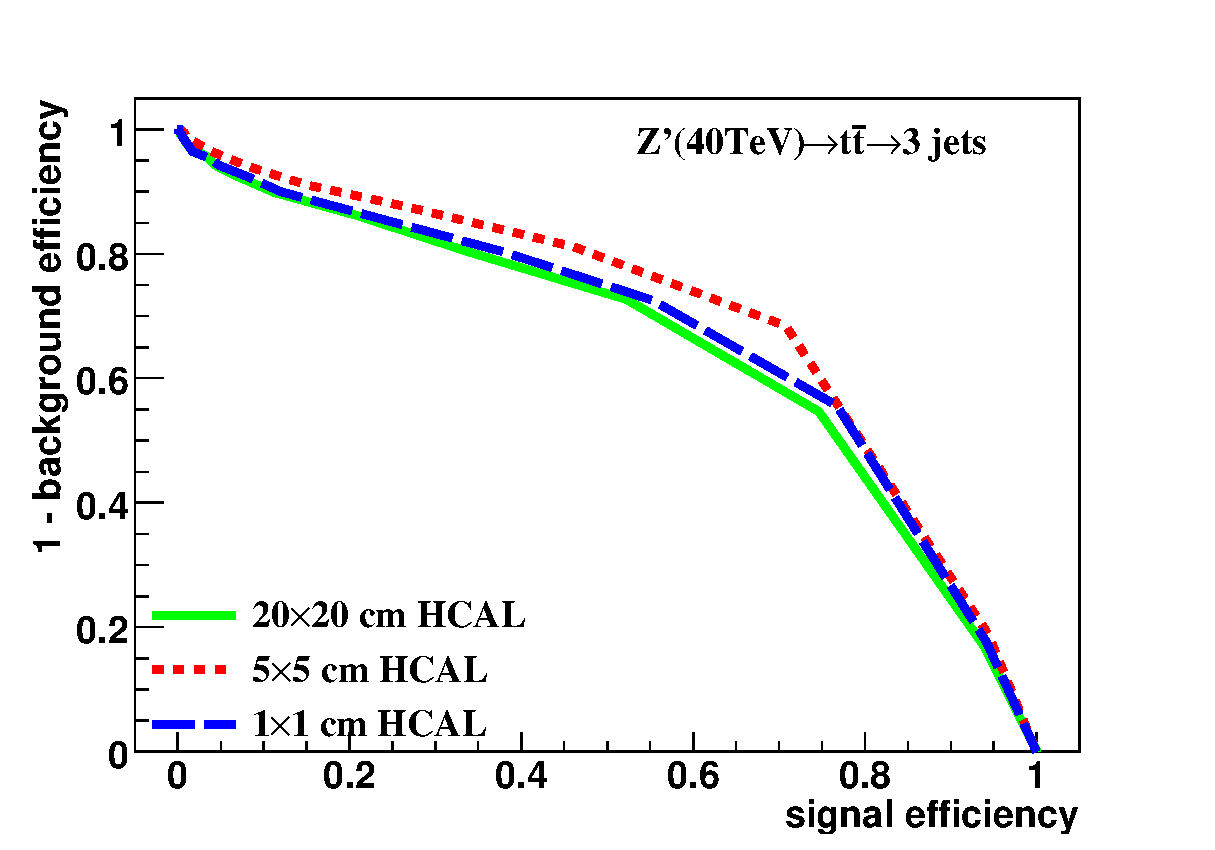
\includegraphics[width=0.43\textwidth]{figs/Rawhit_05GeV_tau32_40tev_04_eff.eps}
   }
\end{center}
\caption{Signal efficiency versus background rejection rate using $\tau_{32}$.The energies of collision at (a)5, (b)10, (c)20, (d)40TeV are shown here. In each picture, the three ROC curves correspond to different detector sizes.}
\label{fig:rawhit_0.5GeV_tau32}
\end{figure}

\section{Studies of signal and background separation using calorimeter hit cut at 0.25GeV}

%25bins
\begin{figure}
\begin{center}
   \subfigure[5 TeV rawhit cut at 0.25GeV] {
   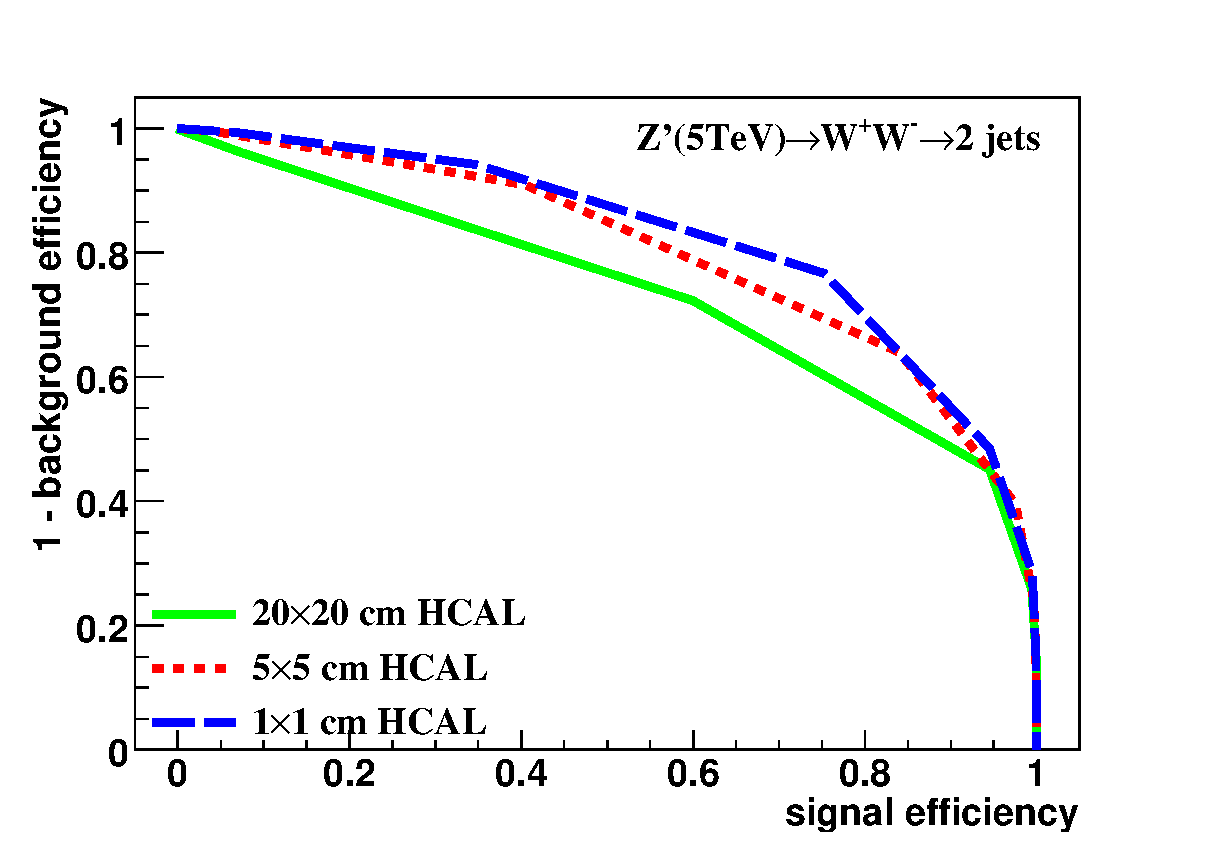
\includegraphics[width=0.43\textwidth]{figs/Rawhit_025GeV_c2b1_5tev_04_eff.eps}\hfill
   }
   \subfigure[10 TeV rawhit cut at 0.25GeV] {
   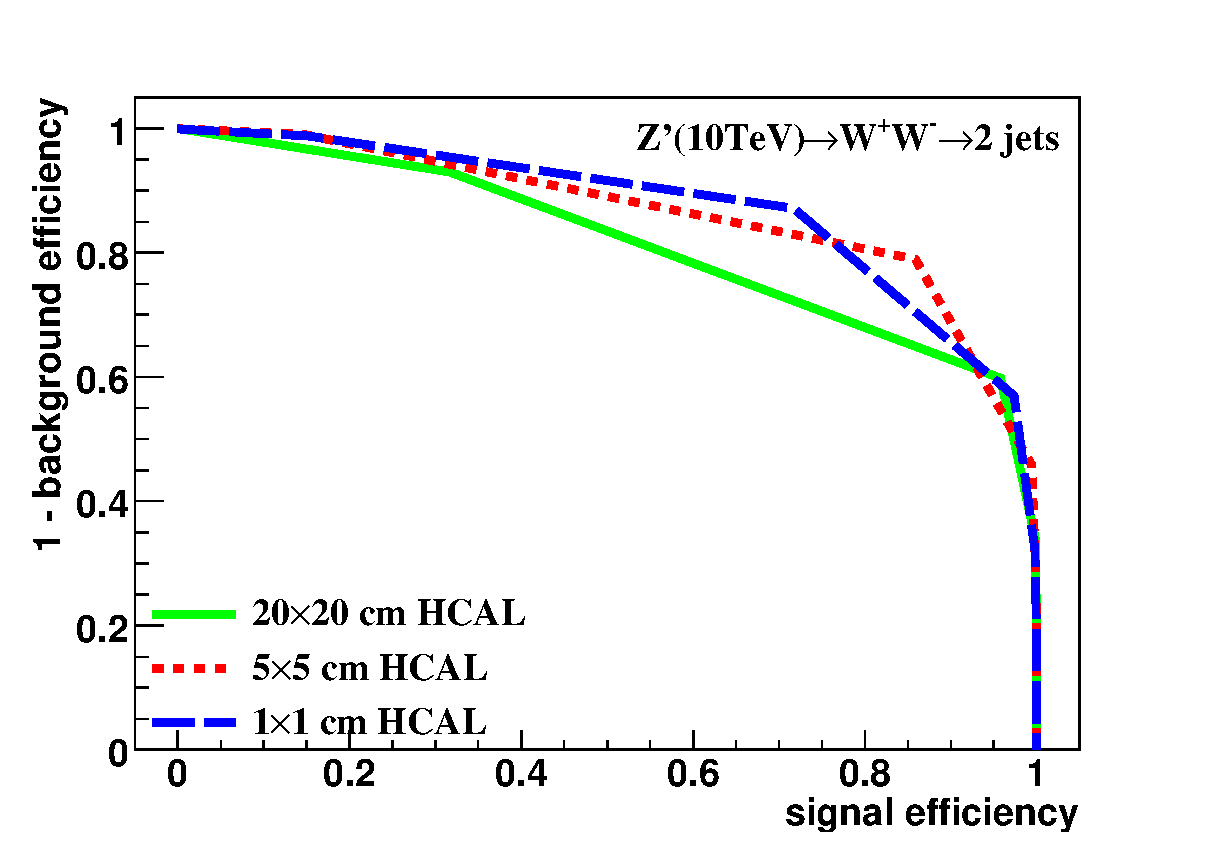
\includegraphics[width=0.43\textwidth]{figs/Rawhit_025GeV_c2b1_10tev_04_eff.eps}
   }
   \subfigure[20 TeV rawhit cut at 0.25GeV] {
   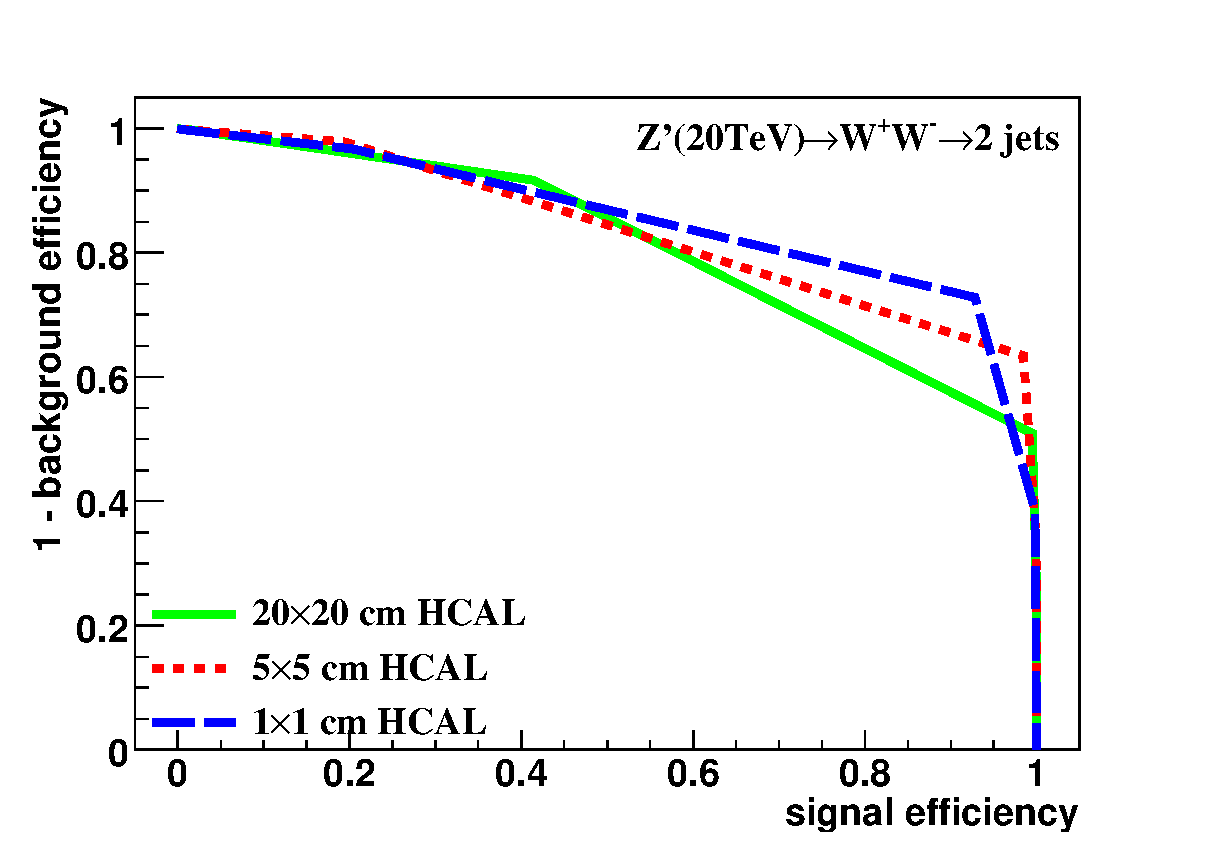
\includegraphics[width=0.43\textwidth]{figs/Rawhit_025GeV_c2b1_20tev_04_eff.eps}
   }
   \subfigure[40 TeV rawhit cut at 0.25GeV] {
   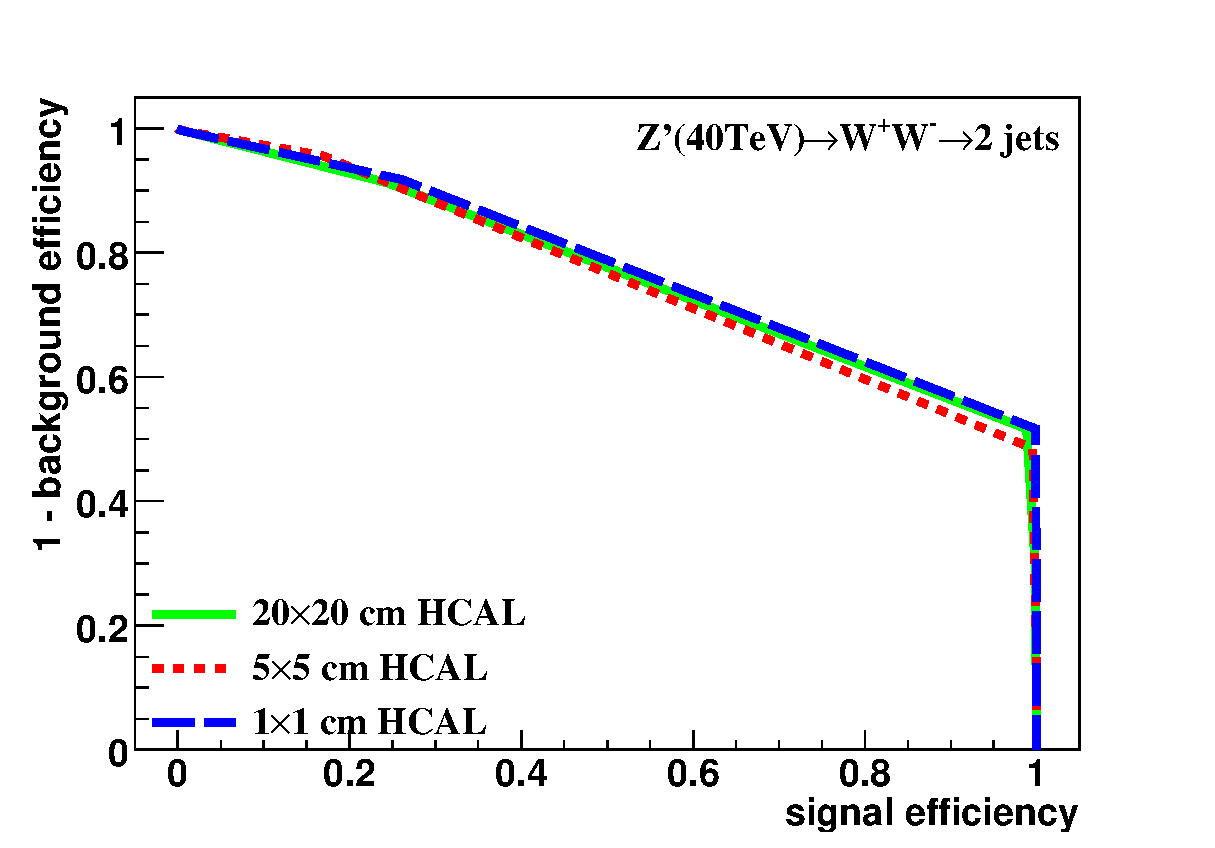
\includegraphics[width=0.43\textwidth]{figs/Rawhit_025GeV_c2b1_40tev_04_eff.eps}
   }
\end{center}
\caption{Signal efficiency versus background rejection rate using $c_2^{(1)}$.The energies of collision at (a)5, (b)10, (c)20, (d)40TeV are shown here. In each picture, the three ROC curves correspond to different detector sizes.}
\label{fig:rawhit_0.25GeV_c2b1}
\end{figure}

%25bins
\begin{figure}
\begin{center}
   \subfigure[5 TeV rawhit cut at 0.25GeV] {
   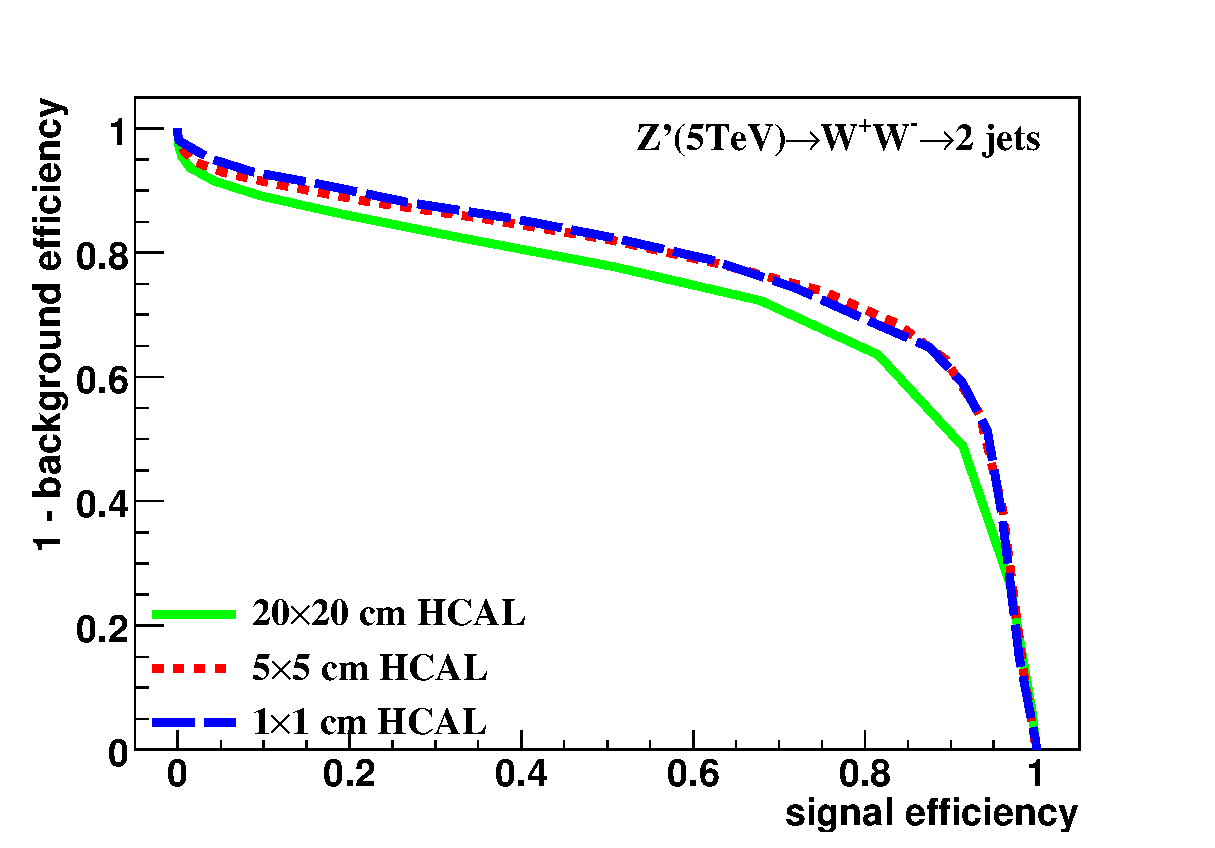
\includegraphics[width=0.43\textwidth]{figs/Rawhit_025GeV_tau21_5tev_04_eff.eps}\hfill
   }
   \subfigure[10 TeV rawhit cut at 0.25GeV] {
   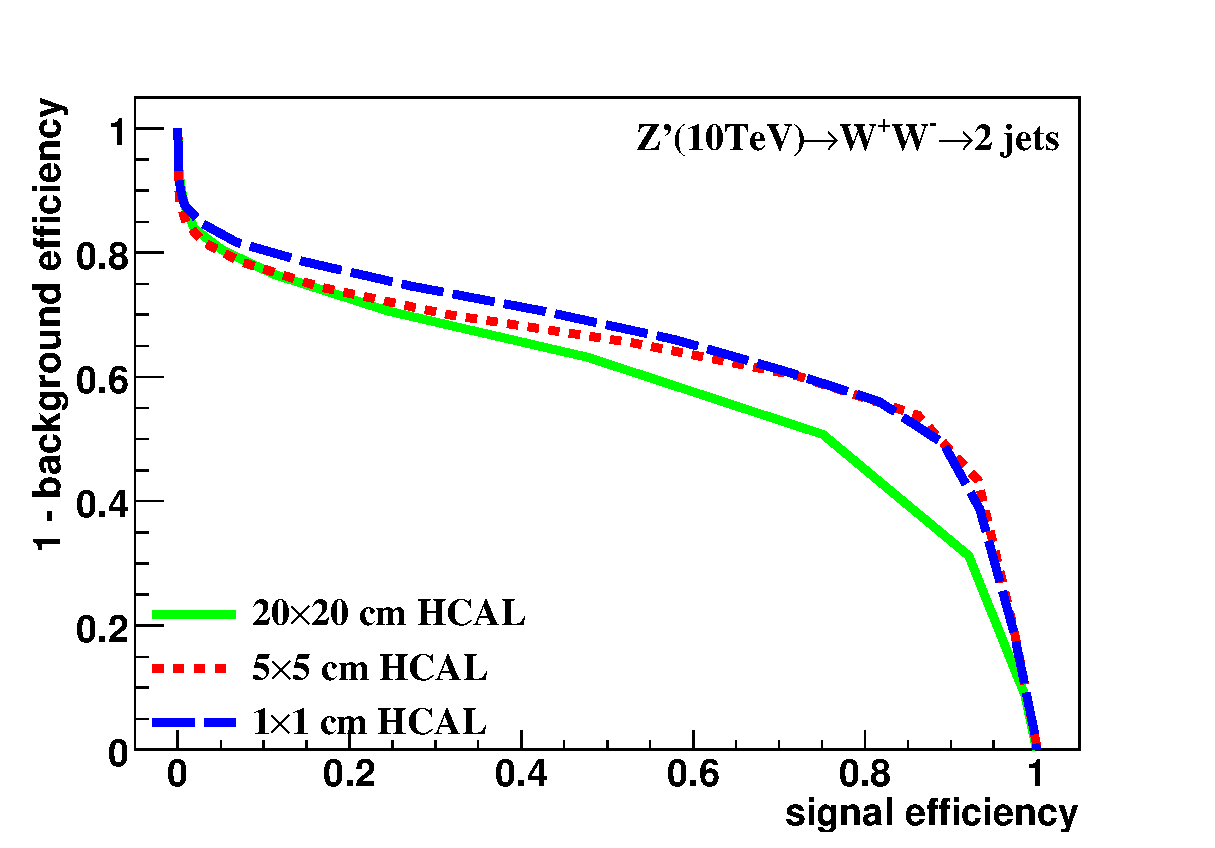
\includegraphics[width=0.43\textwidth]{figs/Rawhit_025GeV_tau21_10tev_04_eff.eps}
   }
   \subfigure[20TeV rawhit cut at 0.25GeV] {
   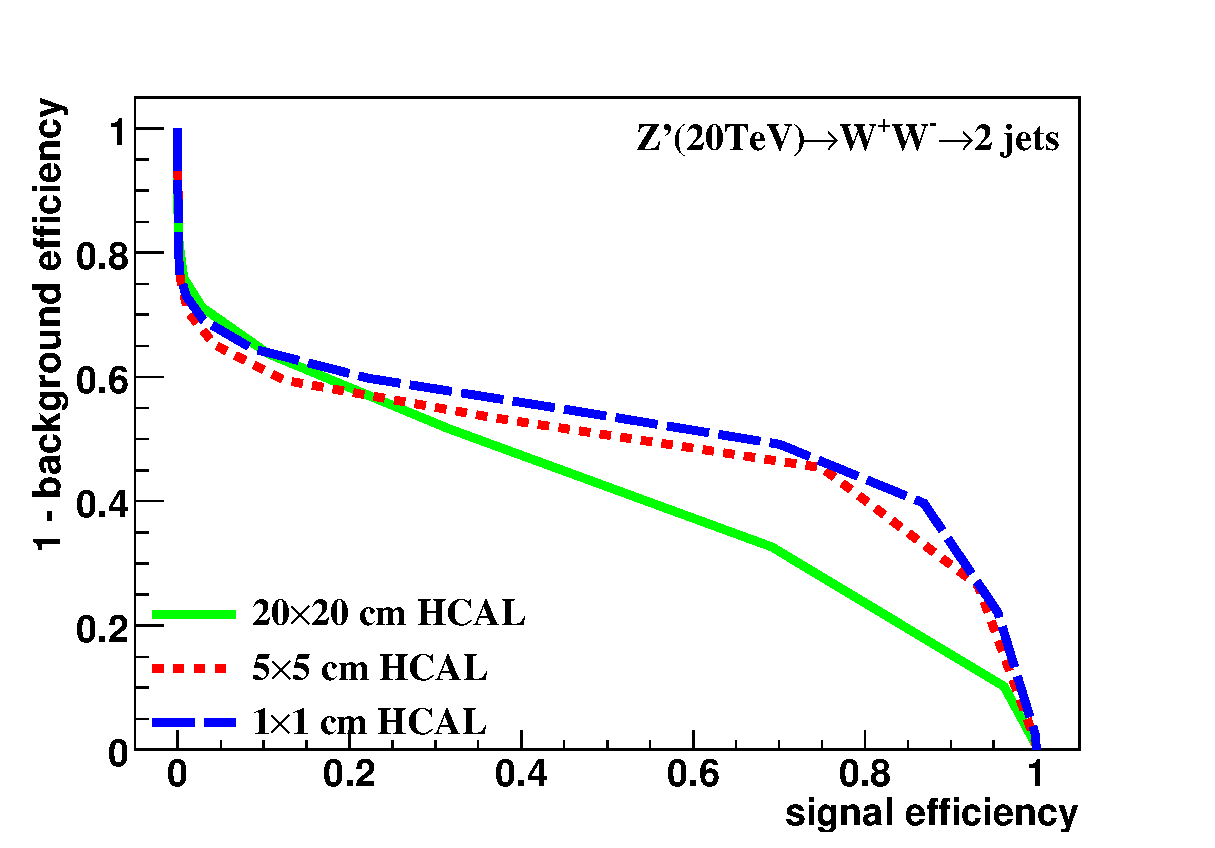
\includegraphics[width=0.43\textwidth]{figs/Rawhit_025GeV_tau21_20tev_04_eff.eps}
   }
   \subfigure[40 TeV rawhit cut at 0.25GeV] {
   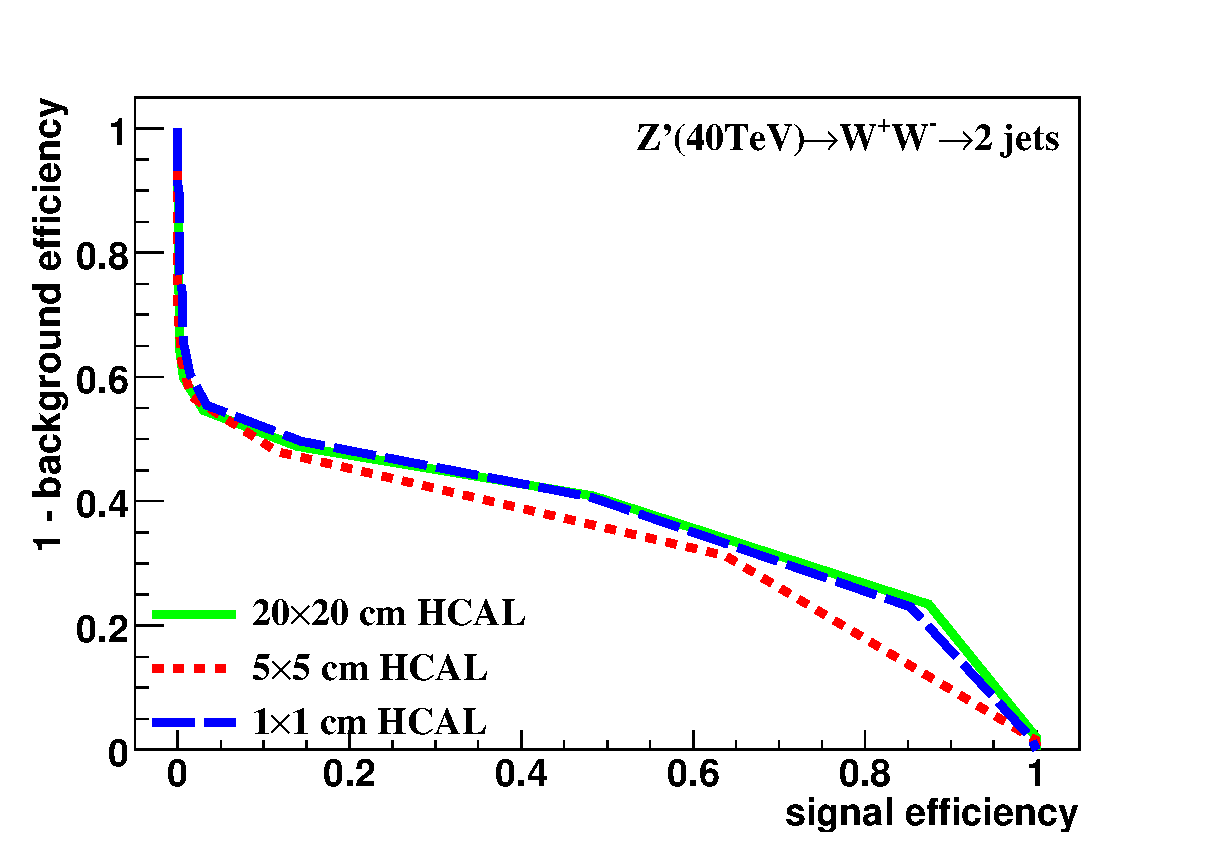
\includegraphics[width=0.43\textwidth]{figs/Rawhit_025GeV_tau21_40tev_04_eff.eps}
   }
\end{center}
\caption{Signal efficiency versus background rejection rate using $\tau_{21}$.The energies of collision at (a)5, (b)10, (c)20, (d)40TeV are shown here. In each picture, the three ROC curves correspond to different detector sizes.}
\label{fig:rawhit_0.25GeV_tau21}
\end{figure}

%25bins
\begin{figure}
\begin{center}
   \subfigure[5 TeV rawhit cut at 0.25GeV] {
   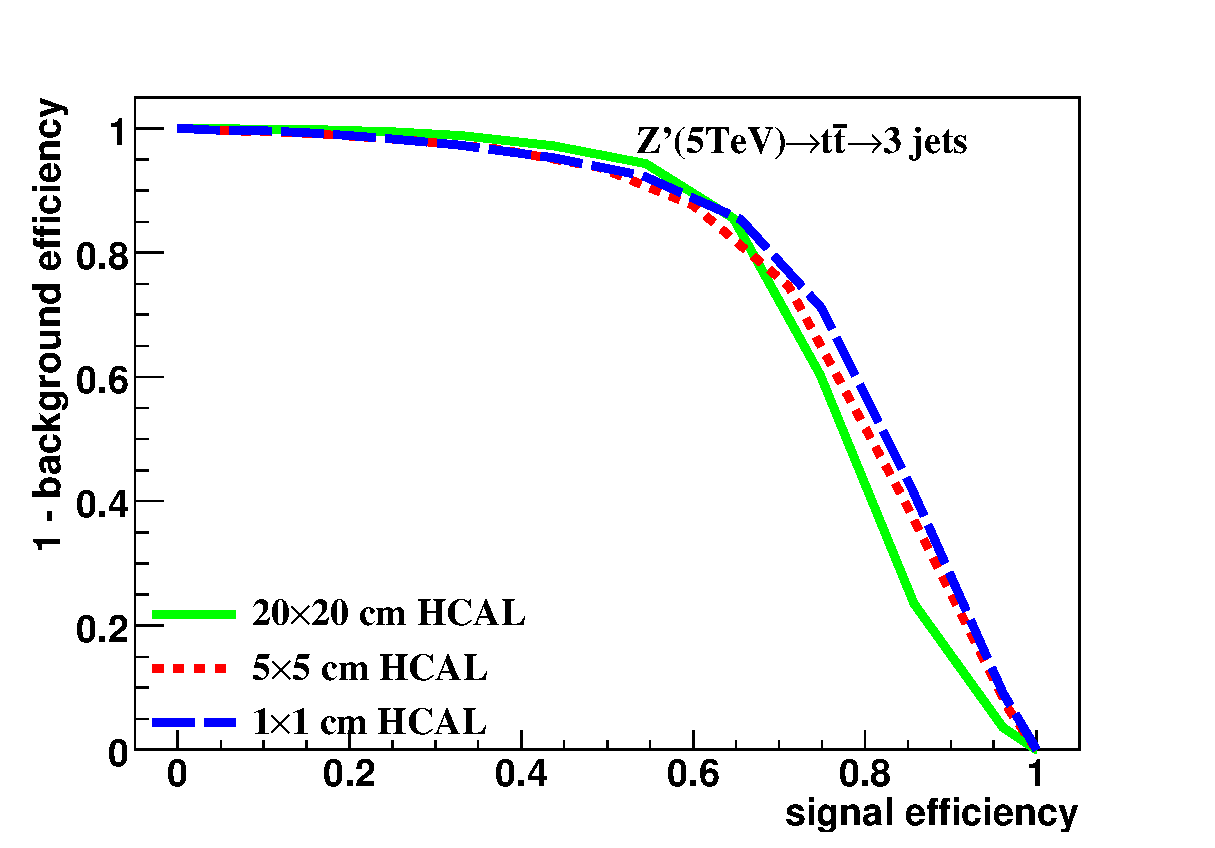
\includegraphics[width=0.43\textwidth]{figs/Rawhit_025GeV_tau32_5tev_04_eff.eps}\hfill
   }
   \subfigure[10 TeV rawhit cut at 0.25GeV] {
   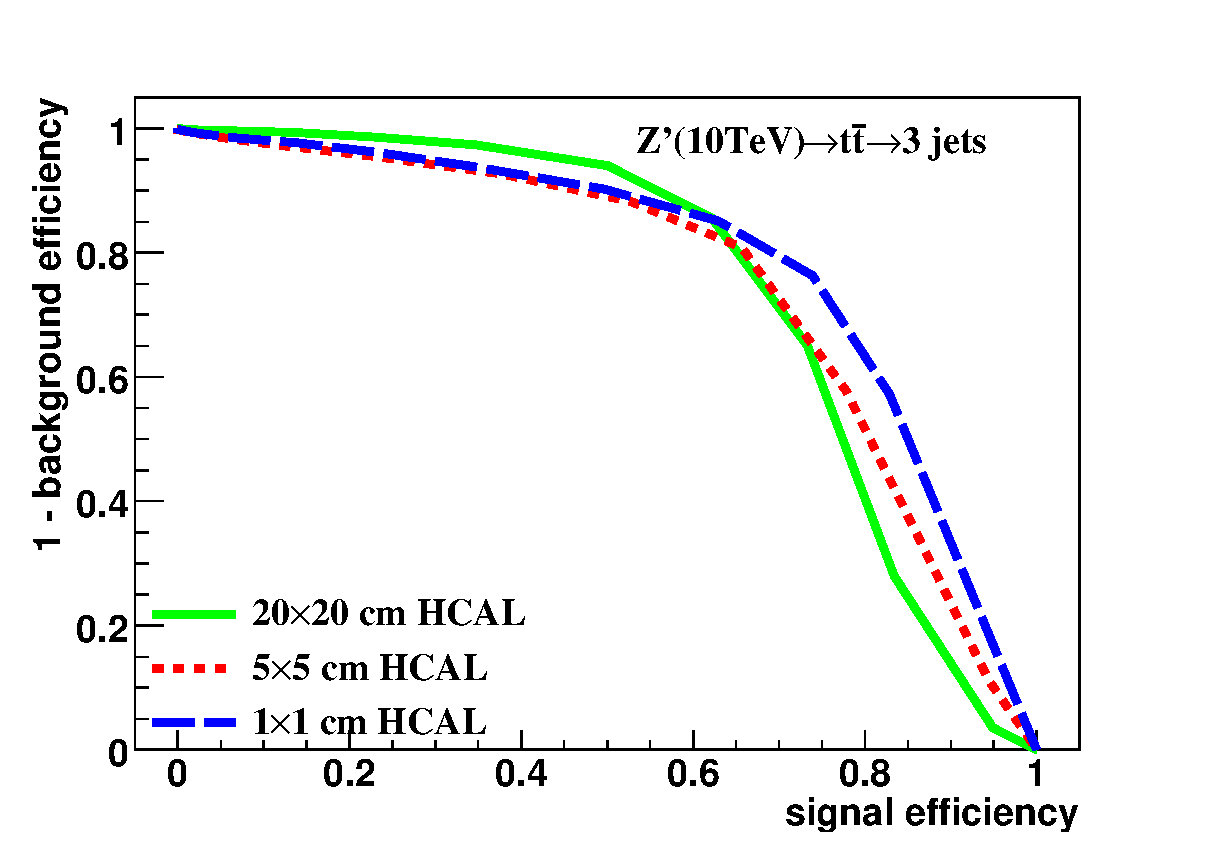
\includegraphics[width=0.43\textwidth]{figs/Rawhit_025GeV_tau32_10tev_04_eff.eps}
   }
   \subfigure[20 TeV rawhit cut at 0.25GeV] {
   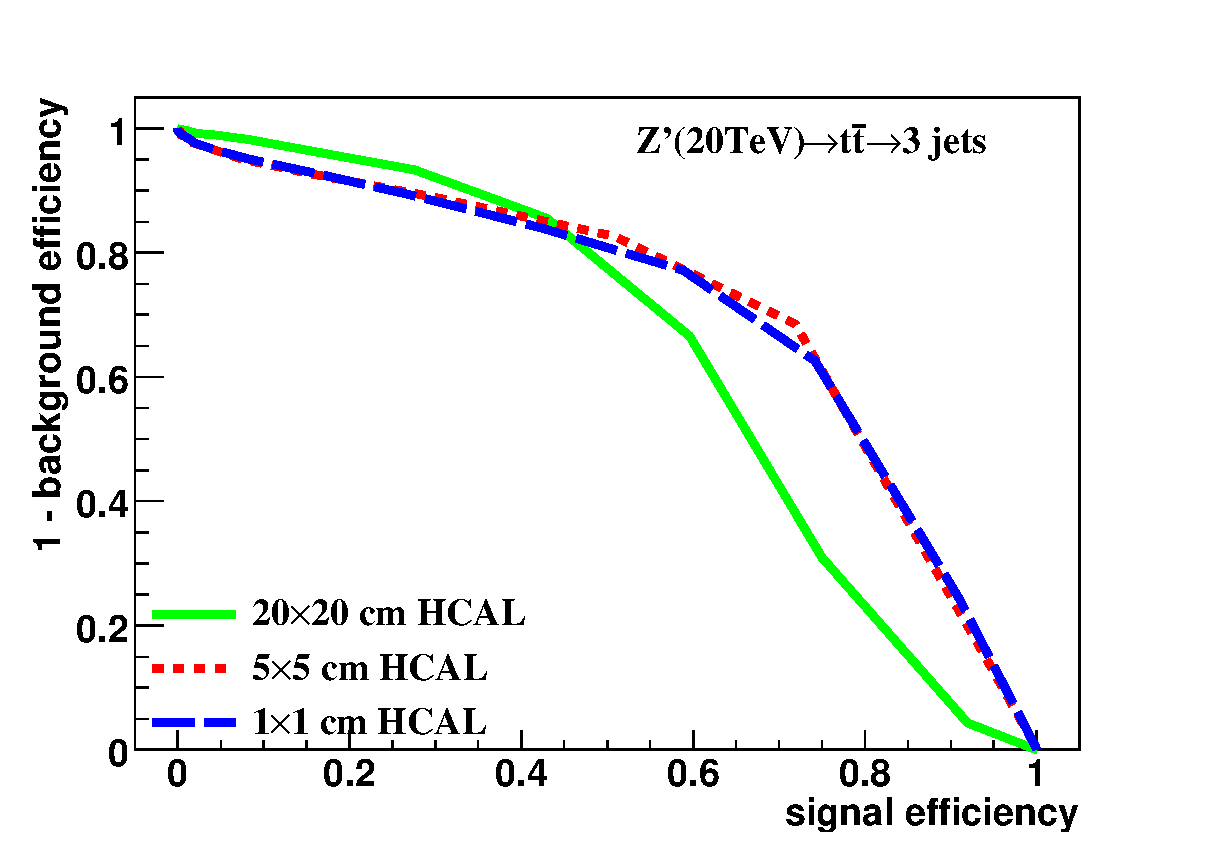
\includegraphics[width=0.43\textwidth]{figs/Rawhit_025GeV_tau32_20tev_04_eff.eps}
   }
   \subfigure[40 TeV rawhit cut at 0.25GeV] {
   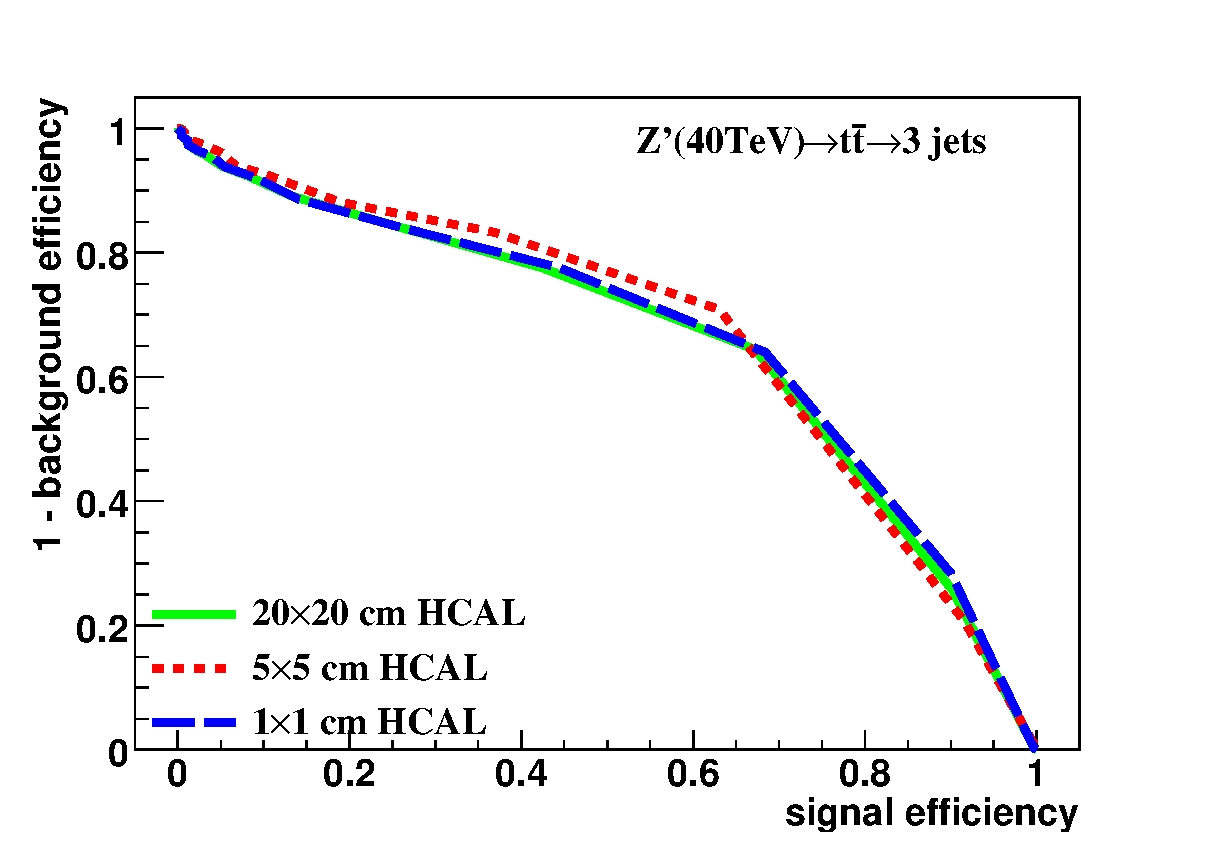
\includegraphics[width=0.43\textwidth]{figs/Rawhit_025GeV_tau32_40tev_04_eff.eps}
   }
\end{center}
\caption{Signal efficiency versus background rejection rate using $\tau_{32}$.The energies of collision at (a)5, (b)10, (c)20, (d)40TeV are shown here. In each picture, the three ROC curves correspond to different detector sizes.}
\label{fig:rawhit_0.25GeV_tau32}
\end{figure}

\section{Studies of signal and background separation using calorimeter hit compare cut at 0.25GeV and cut at 0.5GeV}

%25bins
\begin{figure}
\begin{center}
   \subfigure[5 TeV rawhit cut 0.5GeV compare with cut 0.25GeV] {
   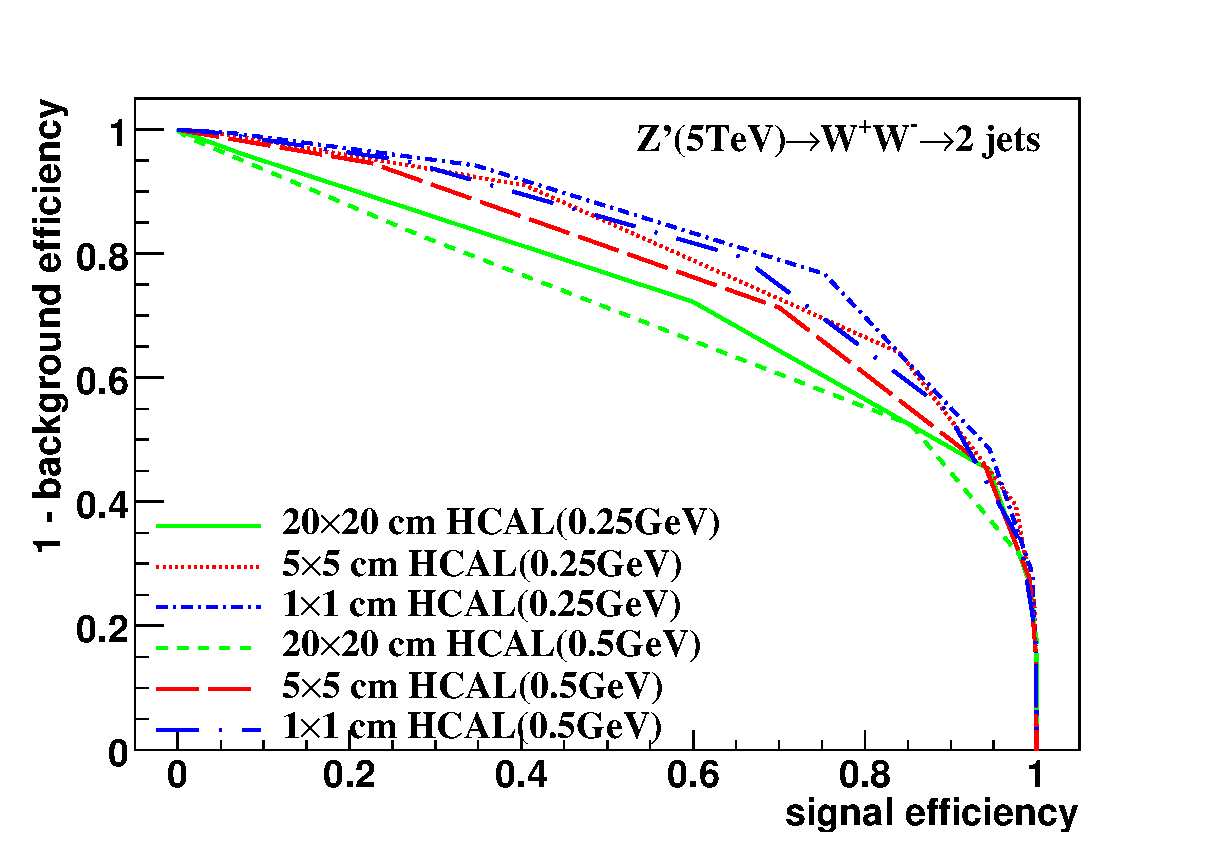
\includegraphics[width=0.43\textwidth]{figs/Rawhit_025GeV_05GeV_c2b1_5tev_04_eff.eps}\hfill
   }
   \subfigure[10 TeV rawhit cut 0.5GeV compare with cut 0.25GeV] {
   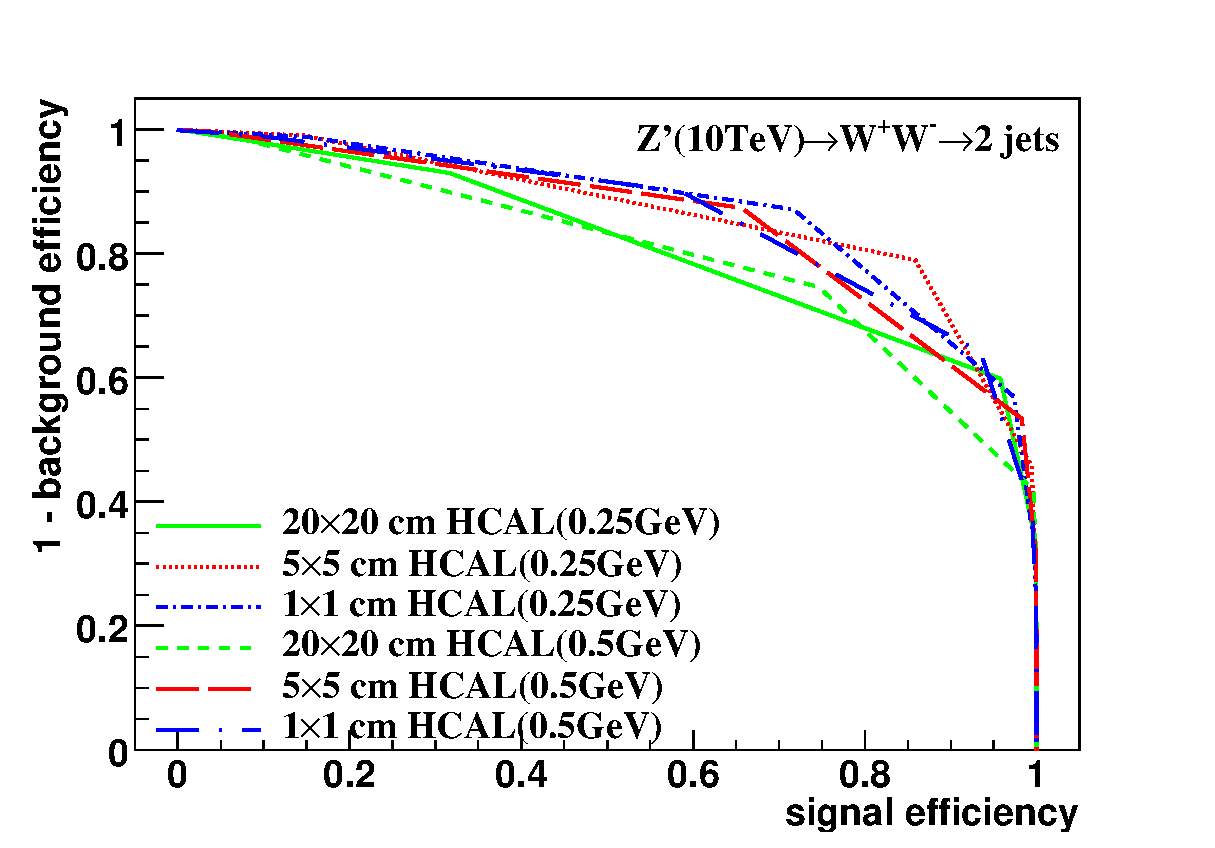
\includegraphics[width=0.43\textwidth]{figs/Rawhit_025GeV_05GeV_c2b1_10tev_04_eff.eps}
   }
   \subfigure[20 TeV rawhit cut 0.5GeV compare with cut 0.25GeV] {
   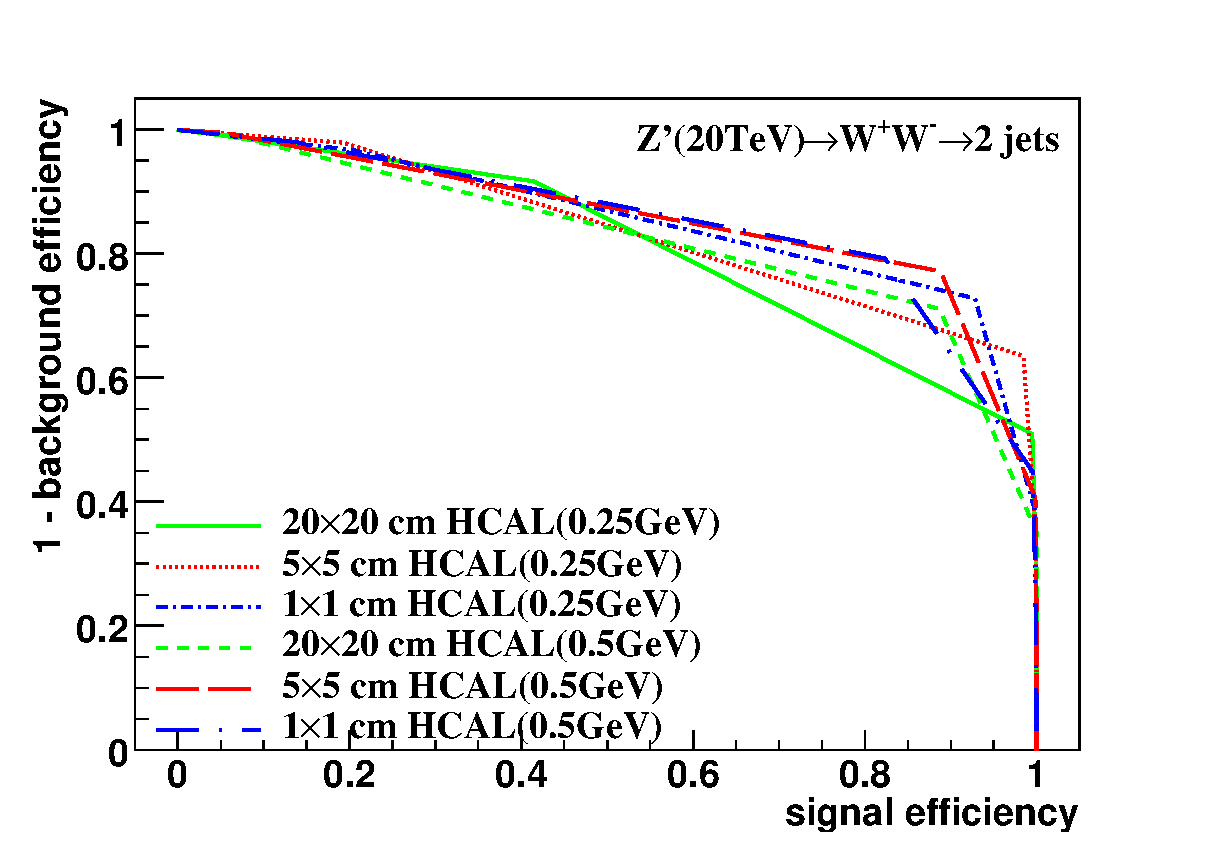
\includegraphics[width=0.43\textwidth]{figs/Rawhit_025GeV_05GeV_c2b1_20tev_04_eff.eps}
   }
   \subfigure[40 TeV rawhit cut 0.5GeV compare with cut 0.25GeV] {
   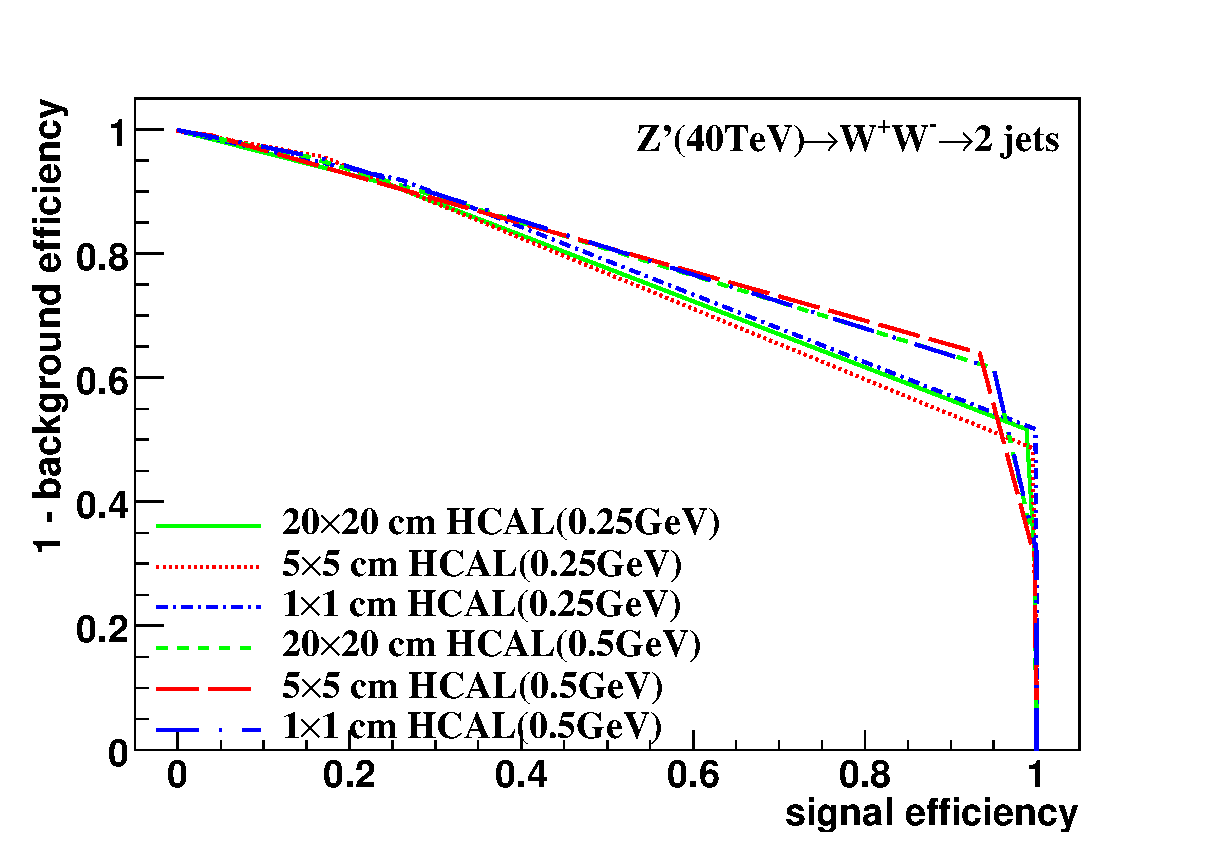
\includegraphics[width=0.43\textwidth]{figs/Rawhit_025GeV_05GeV_c2b1_40tev_04_eff.eps}
   }
\end{center}
\caption{Signal efficiency versus background rejection rate using $c_2^{(1)}$.The energies of collision at (a)5, (b)10, (c)20, (d)40TeV are shown here. In each picture, the six ROC curves correspond to different detector sizes in different cut.}
\label{fig:rawhit_0.5GeV_0.25GeV_c2b1}
\end{figure}

%25bins
\begin{figure}
\begin{center}
   \subfigure[5 TeV rawhit cut 0.5GeV compare with cut 0.25GeV] {
   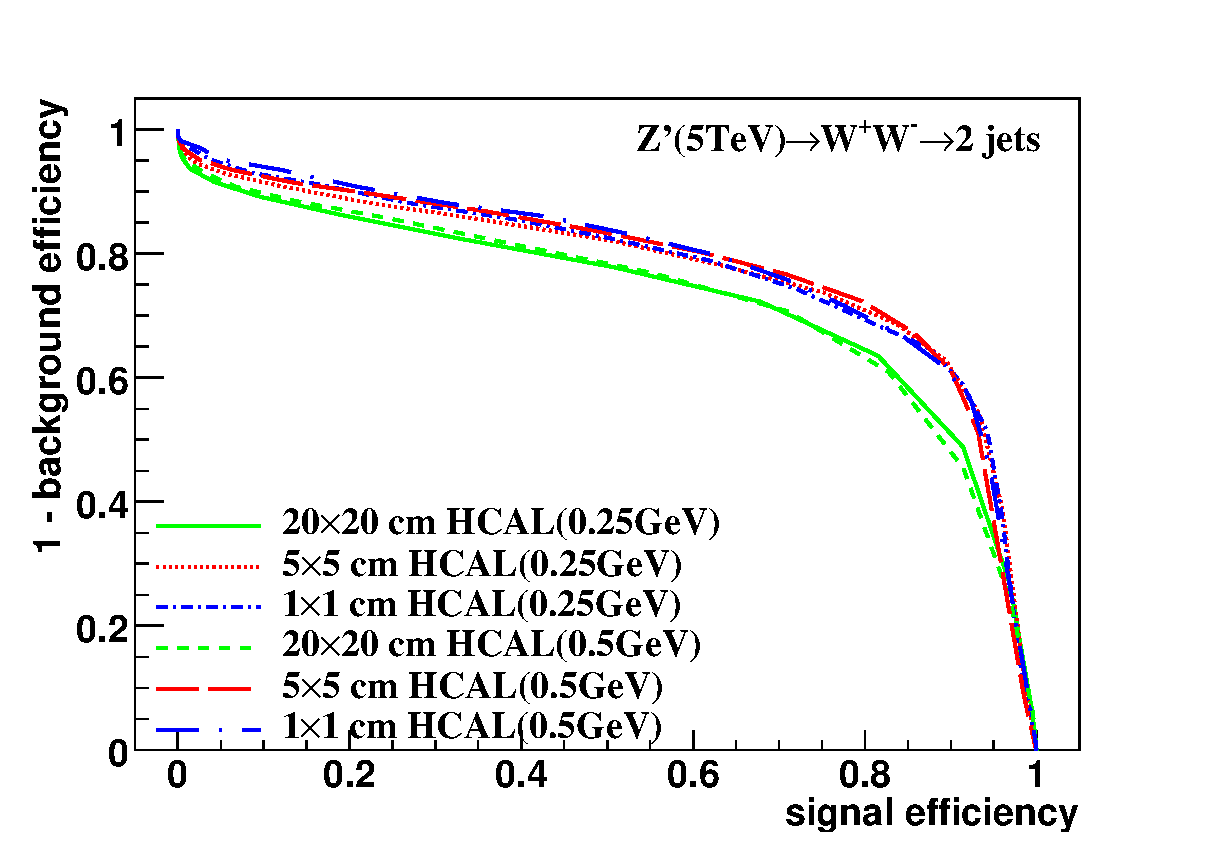
\includegraphics[width=0.43\textwidth]{figs/Rawhit_025GeV_05GeV_tau21_5tev_04_eff.eps}\hfill
   }
   \subfigure[10 TeV rawhit cut 0.5GeV compare with cut 0.25GeV] {
   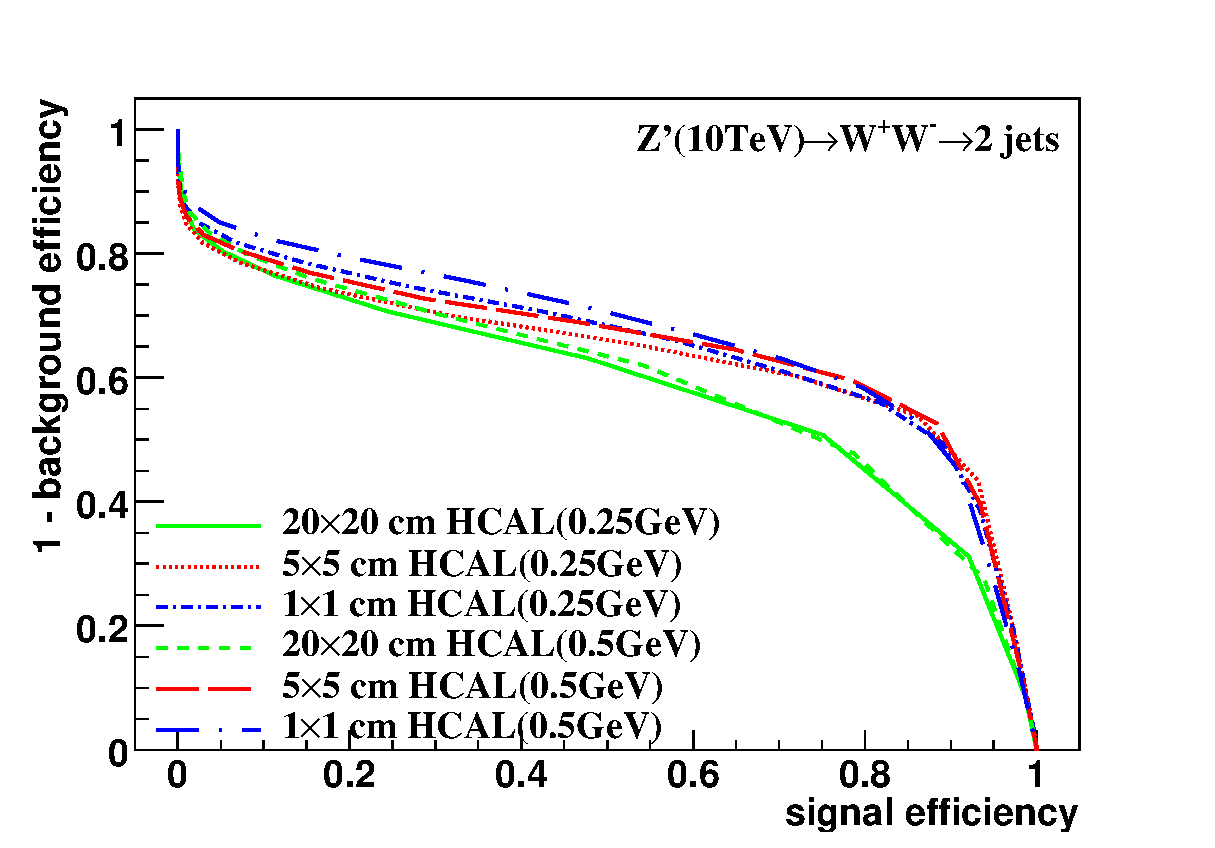
\includegraphics[width=0.43\textwidth]{figs/Rawhit_025GeV_05GeV_tau21_10tev_04_eff.eps}
   }
   \subfigure[20TeV rawhit cut 0.5GeV compare with cut 0.25GeV] {
   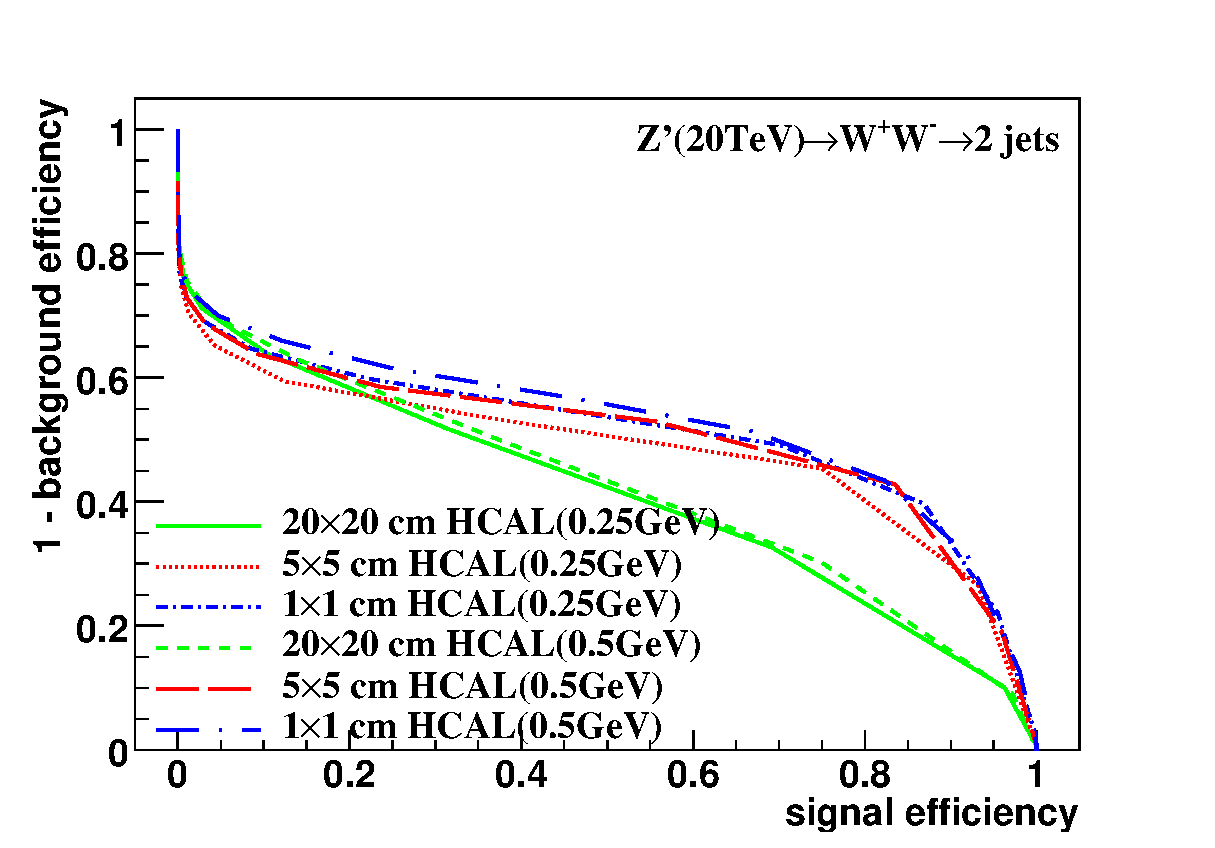
\includegraphics[width=0.43\textwidth]{figs/Rawhit_025GeV_05GeV_tau21_20tev_04_eff.eps}
   }
   \subfigure[40 TeV rawhit cut 0.5GeV compare with cut 0.25GeV] {
   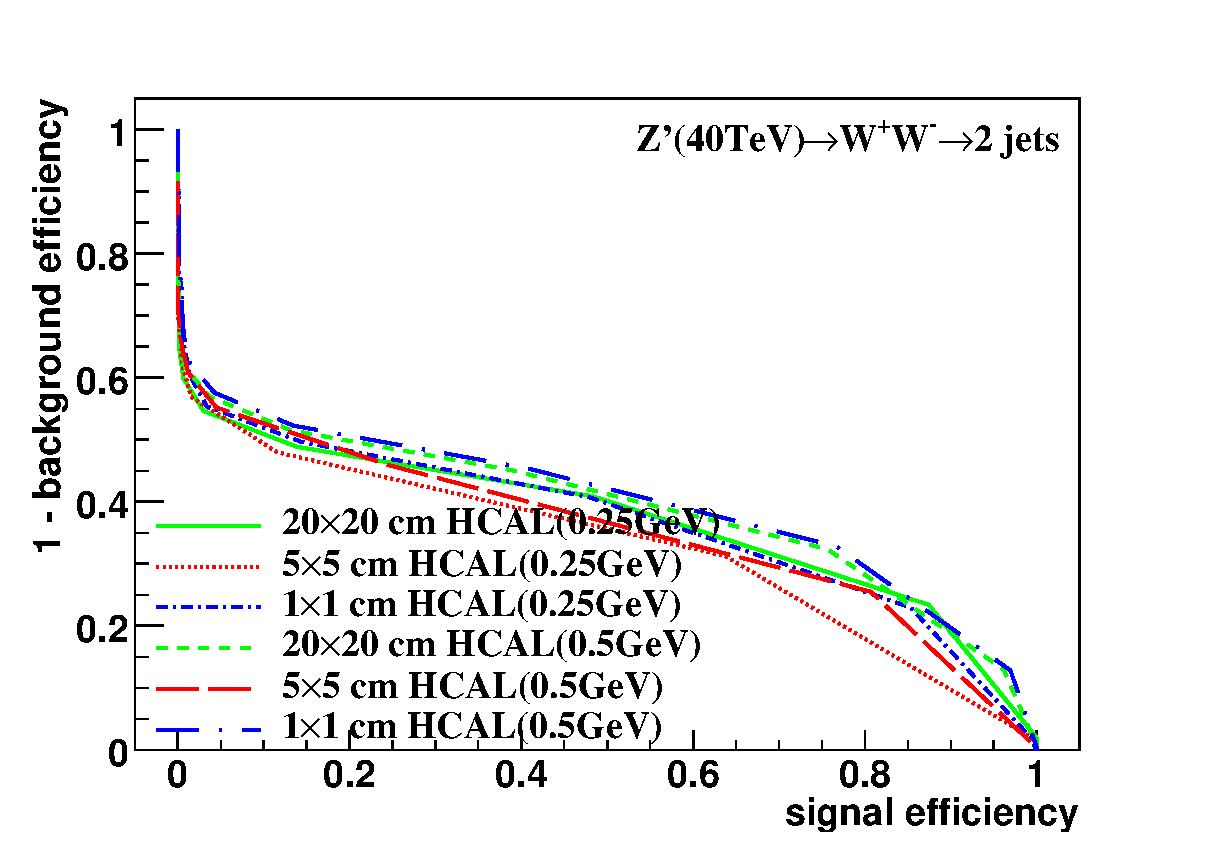
\includegraphics[width=0.43\textwidth]{figs/Rawhit_025GeV_05GeV_tau21_40tev_04_eff.eps}
   }
\end{center}
\caption{Signal efficiency versus background rejection rate using $\tau_{21}$.The energies of collision at (a)5, (b)10, (c)20, (d)40TeV are shown here. In each picture, the six ROC curves correspond to different detector sizes in different cut.}
\label{fig:rawhit_0.5GeV_0.25GeV_tau21}
\end{figure}

%25bins
\begin{figure}
\begin{center}
   \subfigure[5 TeV rawhit cut 0.5GeV compare with cut 0.25GeV]{
   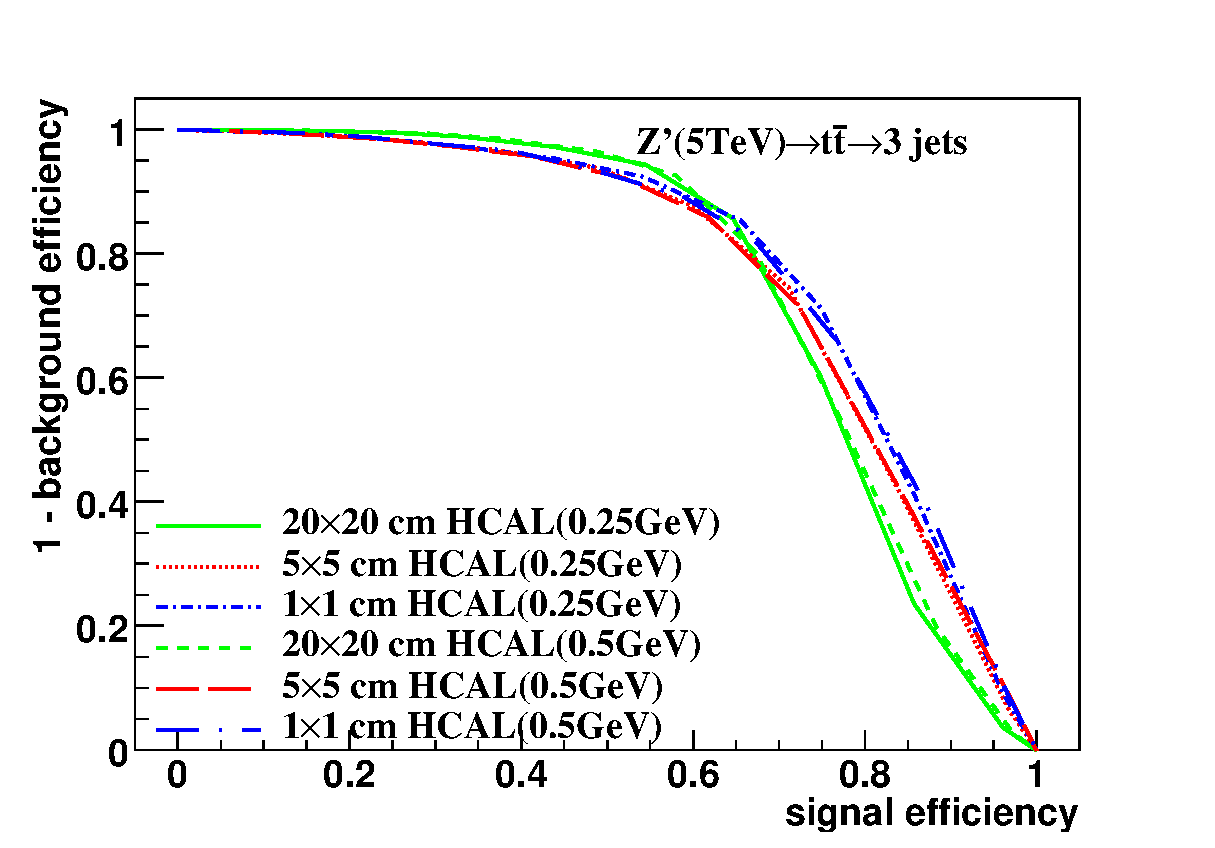
\includegraphics[width=0.43\textwidth]{figs/Rawhit_025GeV_05GeV_tau32_5tev_04_eff.eps}\hfill
   }
   \subfigure[10 TeV rawhit cut 0.5GeV compare with cut 0.25GeV] {
   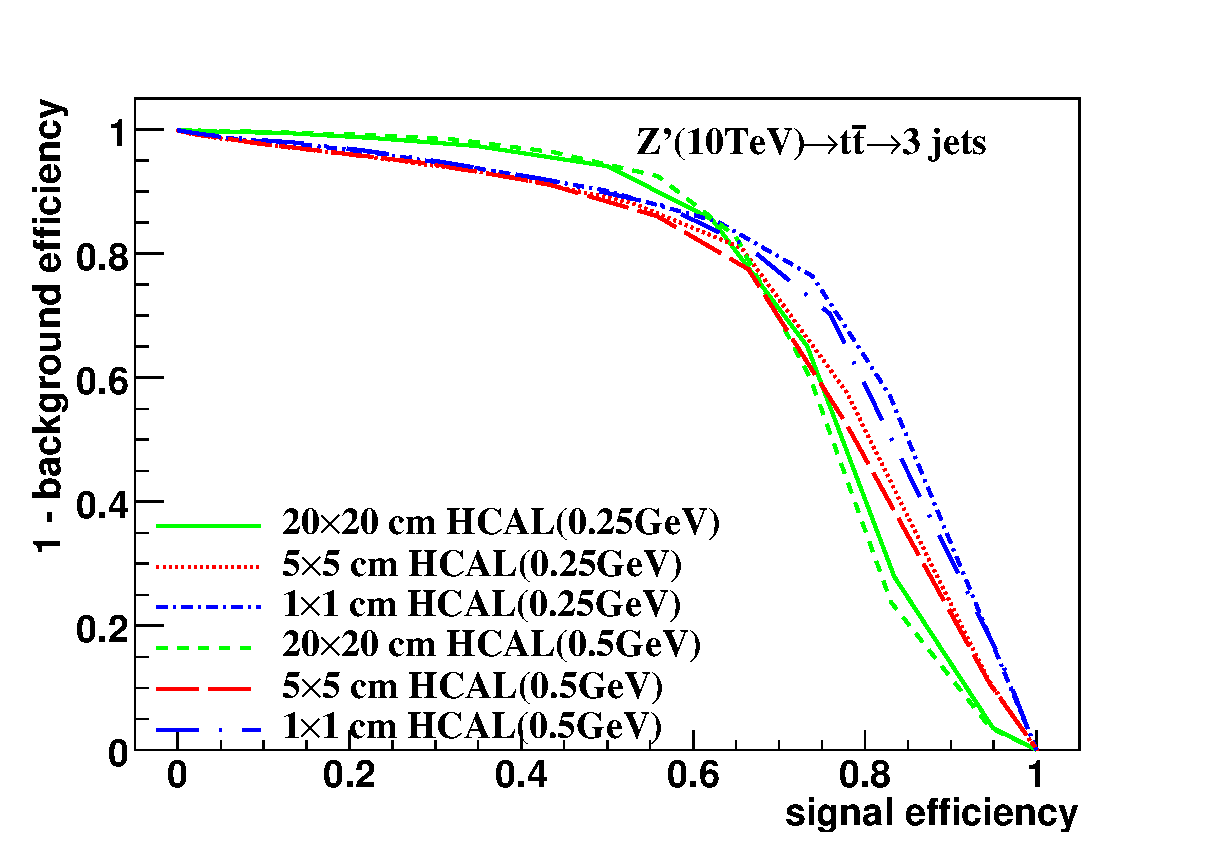
\includegraphics[width=0.43\textwidth]{figs/Rawhit_025GeV_05GeV_tau32_10tev_04_eff.eps}
   }
   \subfigure[20 TeV rawhit cut 0.5GeV compare with cut 0.25GeV] {
   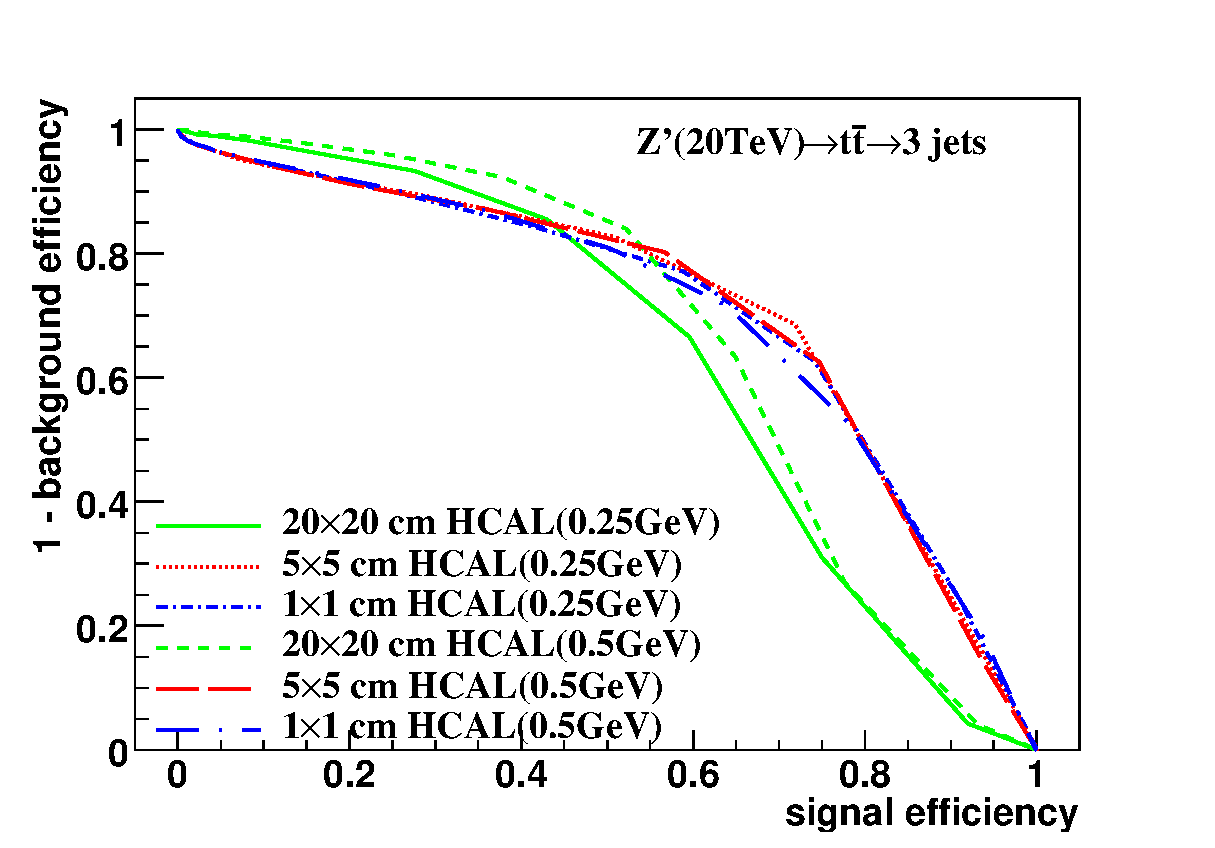
\includegraphics[width=0.43\textwidth]{figs/Rawhit_025GeV_05GeV_tau32_20tev_04_eff.eps}
   }
   \subfigure[40 TeV rawhit cut 0.5GeV compare with cut 0.25GeV] {
   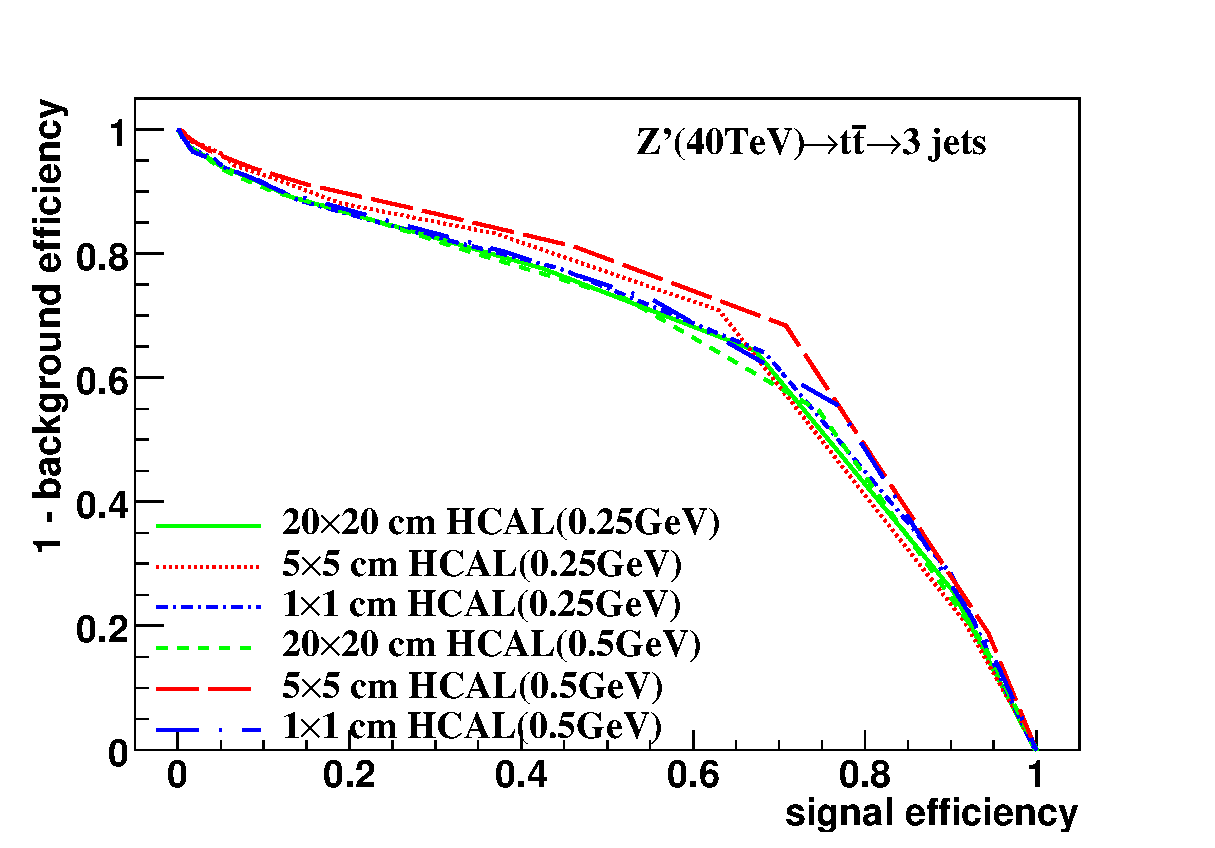
\includegraphics[width=0.43\textwidth]{figs/Rawhit_025GeV_05GeV_tau32_40tev_04_eff.eps}
   }
\end{center}
\caption{Signal efficiency versus background rejection rate using $\tau_{32}$.The energies of collision at (a)5, (b)10, (c)20, (d)40TeV are shown here. In each picture, the six ROC curves correspond to different detector sizes in different cut.}
\label{fig:rawhit_0.5GeV_0.25GeV_tau32}
\end{figure}
\end{document}